\documentclass[a4paper,12pt,parskip,bibtotoc,liststotoc]{article}
    %Festlegung der Dokumentenklasse, zahlreiche Vereinbarungen über Layout, Gliederungsstrukturen,
    %bsp. article -> section, subsection..., book -> chapter, section...
    %parskip = Abstand zwischen Absätzen, Veränderung durch \setlength
\usepackage[utf8]{inputenc}   %Eingabezeichencodierung, die direkte Tastatureingabe von Umlauten ist möglich
\usepackage[ngerman]{babel}     %Neu deutsche Rechtschreibung, Umlaute können geschrieben werden
\usepackage{setspace}           %für Zeilenabstand
\usepackage[notindex,nottoc]{tocbibind}   %Inhaltsverzeichnisse erstellen

%zusätzliche benötigte Pakete
\usepackage{graphicx}           %Graphik
\usepackage{amsmath,amssymb}    %Mathematik
\usepackage{natbib}             %Zitate
\usepackage{marvosym}           %enthält Symbole wie das Eurozeichen
\usepackage{eurosym}
%\setcounter{secnumdepth}{3}
%\setcounter{tocdepth}{3}
\usepackage{footmisc}
\usepackage{listings}
\usepackage{color}
\usepackage{textcomp}
\definecolor{listinggray}{gray}{0.9}
\definecolor{lbcolor}{rgb}{0.9,0.9,0.9}
\lstdefinestyle{befehl}{
	backgroundcolor=\color{lbcolor},
	tabsize=4,
	rulecolor=,
	language=ruby,
        upquote=true,
        aboveskip={0.5\baselineskip},
        columns=fixed,
        showstringspaces=false,
        extendedchars=true,
        breaklines=true,
        prebreak = \raisebox{0ex}[0ex][0ex]{\ensuremath{\hookleftarrow}},
        showtabs=false,
        showspaces=false,
        showstringspaces=false,
        identifierstyle=\ttfamily,
        keywordstyle=\color[rgb]{0,0,1},
        commentstyle=\color[rgb]{0.133,0.545,0.133},
        stringstyle=\color[rgb]{0.627,0.126,0.941}
}

\lstdefinestyle{Listing}{
	frame=single,
	tabsize=4,
        extendedchars=true,
        basicstyle=\footnotesize,
	rulecolor=,
	language=ruby,
        upquote=true,
        aboveskip={0.5\baselineskip},
        columns=fixed,
        showstringspaces=false,
        extendedchars=true,
        breaklines=true,
        prebreak = \raisebox{0ex}[0ex][0ex]{\ensuremath{\hookleftarrow}},
        showtabs=false,
        showspaces=false,
        showstringspaces=false,
        identifierstyle=\ttfamily,
        keywordstyle=\color[rgb]{0,0,1},
        commentstyle=\color[rgb]{0.133,0.545,0.133},
        stringstyle=\color[rgb]{0.627,0.126,0.941}
}

\lstdefinestyle{Listing2}{
	frame=single,
	tabsize=4,
        extendedchars=true,
        basicstyle=\footnotesize,
	rulecolor=,
	language=Java,
        upquote=true,
        aboveskip={0.5\baselineskip},
        columns=fixed,
        showstringspaces=false,
        extendedchars=true,
        breaklines=true,
        prebreak = \raisebox{0ex}[0ex][0ex]{\ensuremath{\hookleftarrow}},
        showtabs=false,
        showspaces=false,
        showstringspaces=false,
        identifierstyle=\ttfamily,
        keywordstyle=\color[rgb]{0,0,1},
        commentstyle=\color[rgb]{0.133,0.545,0.133},
        stringstyle=\color[rgb]{0.627,0.126,0.941}
}

\lstset{literate=%
    {Ö}{{\"O}}1
    {Ä}{{\"A}}1
    {Ü}{{\"U}}1
    {ß}{{\ss}}1
    {ü}{{\"u}}1
    {ä}{{\"a}}1
    {ö}{{\"o}}1
    {~}{{\textasciitilde}}1
}
\usepackage{amsmath}
%\usepackage{mathtools} % lädt auch amsmath
\usepackage{moreverb}

\usepackage{amsthm}
\newtheorem{mydef}{Definition}

\usepackage[table]{xcolor}
\usepackage{colortbl}
\usepackage{multirow}
\usepackage{mdwlist}   %Verringerung Abstand zwischen items -> \begin{itemize*} \end{itemize*}
\usepackage[labelsep=space,justification=centering]{caption}

%\usepackage{hyperref}  %erlaubt Links innerhalb des pdf-Dokuments zu erzeugen

\setlength{\parindent}{0pt}     %Verhinderung des horizontalen Einrückens zu Beginn eines Absatzes

%Seitenlayout
\topmargin -0.9cm       %Vertikaler Abstand der Kopfzeile von der Bezugslinie
\textheight 25cm        %Abstand der Grundlinie der Kopfzeile zum Haupttext
\textwidth 16.5cm       %Breite des Haupttexts
\footskip 1cm           %Abstand der Grundlinien der letzten Textzeile und der Fußzeile
\voffset -0.5cm         %Vertikale Bezugspunktposition
\hoffset -1.2cm         %Horizontale Bezugspunktposition

\onehalfspacing         %anderthalbzeiliger Abstand

\newcommand{\url}{\;}   %URL im Literaturverzeichnis

%eigene Befehlsdefinitionen
\newcommand{\be}{\begin{equation}}     %Mathematische Umgebung
\newcommand{\ee}{\end{equation}}
\newcommand{\bea}{\begin{eqnarray}}
\newcommand{\eea}{\end{eqnarray}}
\newcommand{\bean}{\begin{eqnarray*}}  %ohne Nummerierung
\newcommand{\eean}{\end{eqnarray*}}    %ohne Nummerierung
%%%%%%%%%%%%%%%%%%%%%%%%%%%%%%%%%%%%%%%%%%%%%%%%%%


%%%%%%%%%%%%%%%%%%%%%%%%%%%%%%%%%%%%%%%%%%%%%%%%%%%%%%
%
%    Anfang des Textes
%
%%%%%%%%%%%%%%%%%%%%%%%%%%%%%%%%%%%%%%%%%%%%%%%%%%%%%%
\begin{document}

\pagenumbering{roman}  %römische Seitennummerierung
%%%%%%%%%%%%%%%%%%%%%%%%%%%%%%%%%%%%%%%%%%%%%%%%%%%%%%
%
%    Titelseite
%
%%%%%%%%%%%%%%%%%%%%%%%%%%%%%%%%%%%%%%%%%%%%%%%%%%%%%%
\thispagestyle{empty}  %keine Seitenzahl auf Titelseite
Leibniz Universität Hannover\\
Wirtschaftswissenschaftliche Fakultät\\
Institut für Produktionswirtschaft\\
Prof.\ Dr.\ Stefan Helber

\vspace{5cm}

\begin{center}
Hausarbeit im Rahmen der Veranstaltung \\
Entwicklung von Anwendungssystemen  im WiSe 2014/2015 \\
(Veranstaltungs-Nr. 173610)

\vspace{2.5cm}

%Thema Nr. 5\\[1mm]    %hier Themennummer eintragen
{\Large Entwicklung einer Web-Applikation zur Lösung  \\
des ressourcenbeschränkten Projektplanungsproblems}
\end{center}

\vspace{5.5cm}


\begin{table}[h!]
    \vspace*{-3mm}
    \hspace*{2mm}
  \renewcommand{\arraystretch}{1,5}
    \begin{tabular}{ll}
Andreas Hipp &Robert Matern \\
Ungerstr. 24&Plathnerstr. 49 \\
30451 Hannover&30175 Hannover \\
Matr.-Nr. 3027520 &Matr.-Nr. 2798160 \\[3mm]
Abgabedatum: 24.03.2015
	\end{tabular}
\end{table}

\newpage

%Inhaltsverzeichnis erstellen
\tableofcontents

\newpage  %neue Seite

%Abbildungsverzeichnis erstellen
\listoffigures

\section*{Abkürzungsverzeichnis}
\addcontentsline{toc}{section}{Abkürzungsverzeichnis}
\begin{table}[h!]
    \vspace*{-3mm}
    \hspace*{2mm}
  \renewcommand{\arraystretch}{1,5}
    \begin{tabular}{ll}  %hier die Spaltenausrichtung und Anzahl eintragen
	Admin & Administrator \\         
	GAMS & General Algebraic Modeling System\\
	RCPSP      & Resource-Constrained Project Scheduling \\
	RGL & Ruby Graph Library\\
           RoR & Ruby on Rails \\
	\end{tabular}
\end{table}
%Tabellenverzeichnis erstellen
%\listoftables

%Codeverzeichnis
\newpage
\renewcommand\lstlistlistingname{Quellcodeverzeichnis} 
\lstlistoflistings 
\renewcommand*\lstlistingname{Quellcode} 

\newpage
%Abkürzungsverzeichnis

\newpage
%Symbolverzeichnis
\section*{Symbolverzeichnis}
\addcontentsline{toc}{section}{Symbolverzeichnis}
\begin{table}[h!]
    \vspace*{-3mm}
        \hspace*{2mm}
      \renewcommand{\arraystretch}{1,5}
    \begin{tabular}{ll} 
$d_i$ & Dauer von Vorgang $i$ \\
$FE_i$& frühestes Ende von Vorgang $i$\\
$i,h=1,...,I$ & Vorgänge \\
$k_{ir}$& Kapazitätsbedarf von Vorgang $i$ auf Ressource $r$\\
$kp_r$ & verfügbare Kapazität von Ressource $r$ je Periode\\
$\mathcal{N}_i$ & Menge der direkten Nachfolger von Vorgang $i$ \\
$oc_r$ & Kosten einer Einheit Zusatzkapazität von Ressource $r$ \\
$O_{rt}$ & Zusatzkapazität von Ressource $r$ in Periode $t$ \\
$r=1,...,R$ & Ressourcen \\
$SE_i$& spätestes Ende von Vorgang $i$\\
$t,\tau=1,..., T$ & Perioden\\
$\mathcal{V}_i$ & Menge der direkten Vorgänger von Vorgang $i$ \\
$X_{it}\in\{0,1\}$ & gleich $1$, falls Vorgang $j$ in Periode $t$ endet, sonst $0$
  	\end{tabular}
\end{table}
\newpage
\pagenumbering{arabic}   %ab hier arabische Seitenzahlen beginnend mit 1

%%%%%%%%%%%%%%%%%%%%%%Textteil%%%%%%%%%%%%%%%%%%%%%%%%%%

\section{Einleitung} \label{start}
%Bereits seit mehreren Dekaden spielt Projektarbeit eine wichtige Rolle bei der Aufgabenabwicklung in Wirtschaft und Verwaltung.\footnote{Vgl. \cite{zimmermann2006projektplanung}, S. VI}
Bei einem Projekt handelt es sich um eine zeitlich befristete, relativ innovative und risikobehaftete Aufgabe von erheblicher Komplexität, die meist einer gesonderten Planung bedarf.\footnote{Vgl. \cite{projektdef}} Dementsprechend von großer Bedeutung ist die vorhergehende und genaue Planung von Projekten.\footnote{Vgl. \cite{zimmermann2006projektplanung}, S. VI\label{zum}} Projektplanung ist die Planung aller Arbeitsgänge eines Projekts durch Zuweisung eines Startzeitpunktes, so dass die Zeitbeziehung zwischen den Vorgängen eingehalten und knappe Ressourcenkapazitäten nicht überschritten werden.\footref{zum} Durch das Zerlegen des Projekts in einzelne Arbeitsgänge wird versucht die Komplexität zu reduzieren und eine geordnete Abfolge der Arbeitsgänge zu erstellen, um das Projektziel zu erreichen.\footnote{Vgl. \cite{zimmermann2006projektplanung}, S. 4} Projektziele können dabei unterschiedlich kategorisiert werden, z. B. in Sach-, Termin- oder Kostenziele.\footnote{Vgl. \cite{felkai2011analysieren}, S. 52}\\

Nach DIN 69900 hat ein Arbeitsgang oder ein einzelner Vorgang eines Projekts einen definierten Anfang sowie ein definiertes Ende und dient für das Projekt als Ablaufelement zur Beschreibung eines bestimmten Geschehens.\footnote{Vgl. \cite{69900D}, S. 15} Trotz der Zerlegung besitzen die einzelnen Arbeitsgänge des Projekts eine Beziehung, mit der die Reihenfolge der Ablauffolge bestimmbar ist.\footnote{Vgl. \cite{kellenbrink2014einfuhrung}, S. 6-7} Oft wird zur Darstellung der Vorgangsrelationen ein Vorgangsknoten-Netzplan verwendet.\footnote{?????} %D. h. es können nur Arbeitsgänge abgeschlossen werden, wenn deren notwendigen Vorgänge bereits abgeschlossen wurden. Ein einfaches Beispiel wäre die sogenannte Hochzeit in der Automobilherstellung. Sobald Karosserie und Motor eines Fahrzeugs hergestellt wurden, können diese zwei Elemente in einem nachfolgenden Prozess verbunden werden.
Ein Arbeitsgang ist i. d. R. verbunden mit dem Einsatz von Ressourcen, welche wiederum mit Kosten verbunden sind. Eine Möglichkeit, das Projektziel unter minimaler Ressourcenverwendung zu erreichen, ist die effiziente Planung der Ablauffolge der Arbeitsgänge eines Projekts.\footnote{Vgl. \cite{bartels2009projektplanung}, S. 11-12} Damit ist es möglich, mehrere Projekte bei einer gegebenen Zeitvorgabe unter Einhaltung von Ressourcenrestriktionen fertigzustellen bzw. bei konstanter Ressourcenkapazität ein Projekt in kürzerer Zeit abzuschließen. \\

Zur Bestimmung der optimalen Ablauffolge der einzelnen Arbeitsgänge eines Projekts kann ein Optimierungsmodell verwendet werden, mit dem für eine festgelegten Ablauffolge eines Projekts und unter Berücksichtigung der Ressourcenbeschränkung die Fertigstellungszeit minimiert wird. Im Kapitel \ref{Grund} wird eine solche Modellformulierung für das ressourcenbeschränkte Projektplanungsproblem als sogenannte Kapazitätsplanung vorgestellt.\footnote{????} Alternativ wird in dem Kapitel das Optimierungsmodell um die Bedienung erweitert, dass  Zusatzkapazitätseinheiten gebucht werden können. Mit dieser Modellerweiterung wird von der Kostenplanung in Projekten gesprochen. Bezeichnet wird im Allgemeinen das ressourcen-beschränkte Projektplanungsproblem  mit der englischen Bezeichnung des \textit{Resource-Con\-strained Project Scheduling Problem (RCPSP)}. Bei dem RCPSP handelt es sich um eine abstrakte mathematische Modellformulierung. Ziel der vorliegenden Arbeit ist es das RCPSP in Ruby on Rails (RoR) zu implementieren. Bei RoR handelt es sich um ein Framework zur Entwicklung von Webdokumenten bzw. Internetseiten.\footnote{???} Es baut auf der Programmiersprache Ruby auf und ist ursprünglich von David Heinemeier Hansson entwickelt.\footnote{???} Die Implementierung bedarf einer Verknüpfung von RoR und GAMS\footnote{General Algebraic Modeling System}. Unter GAMS wird eine algebraische Modellierungssprache für mathematische Optimierungsprobleme verstanden, mit der das RCPSP gelöst wird.\footnote{???} Im Kapitel \ref{Haupt} wird die Entwicklung des Anwendungssystems zum Lösen des RCPSP ausführlich beschrieben. Ergänzt wird diese Arbeit durch eine kritische Würdigung des Anwendungssystems in Kapitel \ref{krit} sowie einem Fazit in Kapitel \ref{Fazit}.

\section{Grundlagen zur ressourcen-beschränkten Projektplanung und zu dem Framework Ruby on Rails} \label{Grund}
\subsection{Kapazitätsplanung}
Ein Großteil an Projekten besitzt die Eigenschaft eines beschränkten Ressourcenkontingents.\footnote{Vgl. \cite{kellenbrink2014einfuhrung}, S. 11} Soll demgemäß die vorgegebene Terminierung des Projektes als zuvor festgesetztes Ziel erreicht werden, muss neben der Reihenfolgerestriktion auch der Ressourcenbedarf der unterschiedlichen Arbeitsgänge sichergestellt werden. Mit der Einhaltung des Ressourcenbedarfs ist es möglich, alle zur Erfüllung des Projektes notwendigen Arbeitsgänge auszuführen und somit letztendlich das Projekt abzuschließen. Neben limitierten Ressourcen, die während des gesamten Projekts nur ein Mal zur Verfügung stehen, wie bspw. das Projektbudget, gibt es Ressourcen, die nach einer bestimmten Anzahl von Perioden erneuert werden können.\footnote{Vgl. \cite{neumann2003project}, S. 21-22} Erneuerbare Ressourcen sind bspw. die Produktionskapazität einer Maschine oder der Personaleinsatz für ein Projekt. In dieser Arbeit wird der Fokus auf diese erneuerbaren Ressourcen gelegt.\\

Zur Lösung des ressourcenbeschränkten Projektplanungsproblems kann das Modell RCPSP genutzt werden. Das RCPSP legt durch Fixierung der Aktivitätsstartzeitpunkte den Projektgrundablauf zur Zielerreichung der Minimierung der Projektdauer fest. Dies geschieht unter Einhaltung der Startzeitpunkt- bzw. der Vorrangsbedingung der einzelnen Arbeitsgänge sowie der Kapazitätsbeschränkung der erneuerbaren Ressourcen.\footnote{Vgl. \cite{demeulemeester2011robust}, S. 23} Die im folgenden aufgestellte Zielfunktion des RCPSP zur Minimierung der Projektdauer ist die gängige Version der Kapazitätsplanung,\footnote{Vgl. \cite{drexl1997neuere}, S. 98} andere Variationen sind aber ebenfalls möglich.\footnote{Vgl. \cite{talbot1982resource}, S. 1200}\\

Nachfolgend wird das deterministische RCPSP in diskreter Zeit formuliert.\footnote{????} Charakteristisch für eine mathematische Modellformulierung in diskreter Zeit sind die Zeiteinheiten, die den Perioden $t, \tau$ entsprechen.\\

\textbf{Modell RCPSP}
\begin{eqnarray} \label{Ziel}
\min Z = \sum_{t=FE_{I}}^{SE_{I}}t \cdot X_{I,t}\hfill  
\end{eqnarray}

unter Beachtung der Restriktionen
\begin{multline} \label{N1}
\sum_{t=FE_{i}}^{SE_{i}} X_{it} = 1
\hfill   i = 1,...,I
\end{multline}\vspace{-3.0ex}

\begin{multline} \label{N2}
\sum_{t=FE_{h}}^{SE_{h}}t \cdot X_{ht} \leq \sum_{t=FE_{i}}^{SE_{i}}(t - d_{i}) \cdot X_{it}
\hfill   i =1,...,I;\; h \in \mathcal{V}_{i}
\end{multline}\vspace{-3.0ex}

\begin{multline} \label{N3}
\sum_{i=1}^{I}\sum_{\tau=\max(t,FE_{i})}^{\tau=\min(t+d_i-1,SE_i)}k_ {ir} \cdot X_{i\tau} \leq kp_{r}
\hfill   r =1,...,R;\; t=1,...,T
\end{multline}\vspace{-3.0ex}
\begin{multline} \label{N4}
X_{it} \in \{0,1\}
\hfill   i \in \mathcal{I};\; t \in \{FE_{i},...,SE_{i}\}\end{multline}\vspace{-6.0ex}\\

Es wird ein Projekt betrachtet, dass aus $I$ unterschiedlichen Arbeitsgängen besteht. Jeder Arbeitsgang $i$ hat eine definierte Menge von zu erledigenden Vorgängerarbeitsgängen $h \in \mathcal{V}_{i}$. Des Weiteren ist für die Fertigstellung des Projekts die Abarbeitung der Arbeitsgänge in topologischer Reihenfolge notwendig. D. h. der Vorgänger $h$ hat stets eine kleinere Ordnungszahl als sein Nachfolger $i\;(h<i)$ und muss zur Fortsetzung des Projektverlaufs beendet sein. Die Bearbeitungsdauer eines Arbeitsgangs $i$ wird mit dem Parameter $d_{i}$ festgelegt.  Bei dem RCPSP in diskreter Zeit wird die Annahme getroffen, dass die Dauer durch einen ganzzahligen Parameter abgebildet wird. Der Startzeitpunkt des Projekts ist $t = 0$ und erstreckt sich über einen Gesamtzeitraum von $T$ Perioden. Um die Reihenfolgebedingungen einzuhalten, werden einem Projekt zwei Dummy-Arbeitsgänge \glqq Beginn\grqq\;($i=1$) und \glqq Ende\grqq\;($i=I$) hinzugefügt, welche mit einer Dauer von $0$ Zeiteinheiten bewertet werden.\footnote{Vgl. \cite{zimmermann2006projektplanung}, S. 66} Dadurch wird der Projektbeginn und das Projektende exakt terminiert. Der Parameter $k_{ir}$ stellt die benötigten Kapazitäten der erneuerbaren Ressource $r$ bei der Durchführung von Arbeitsgang $i$ dar. Die Ressourcen $r \in R$ sind in einer Periode innerhalb des Umfangs ihrer Kapazität $kp_{r}$ nutzbar. Da es sich um erneuerbare Ressourcen handelt, stehen diese zu jeder neuen Periode in vollem Umfang erneut zur Verfügung. Ungenutzte Ressourcen sind jedoch nicht auf nachfolgende Arbeitsgänge und Perioden übertragbar.\footnote{Vgl. \cite{kellenbrink2014einfuhrung}, S. 12} Um den Fertigstellungszeitpunkt der einzelnen Arbeitsgänge $i$ festlegen zu können, wird der Modellformulierung in diskreter Zeit die binäre Entscheidungsvariable $X_{it}$ hinzugefügt.\footnote{Vgl. \cite{pritsker1969multiproject}, S. 94} Diese Binärvariable nimmt den Wert $1$ an, falls der Arbeitsgang $i$ zum Zeitpunkt $t$ beendet wird.\\

Mittels der Zielfunktion \eqref{Ziel} wird der Fertigstellungszeitpunkt des Projekts minimiert. Dafür wird der Zeitraum zwischen dem frühesten und spätesten Fertigstellungszeitpunkt $FE_{I}$ und $SE_{I}$ aller durchzuführenden Arbeitsgänge $I$ betrachtet. Nebenbedingung \eqref{N1} stellt sicher, dass ein Arbeitsgang $i$ zwischen dem jeweiligen für diesen Arbeitsgang geltenden frühesten und spätesten Fertigstellungszeitpunkt nur exakt ein Mal durchgeführt wird. Die Reihenfolgerestriktion wird mit der Nebenbedingung \eqref{N2} eingehalten. Sie stellt sicher, dass jeder Vorgänger $h \in \mathcal{V}_{i}$ beendet ist, bevor der Arbeitsgang $i$ startet. Der Term $(t - d_{i})$ garantiert für den Arbeitsgang $i$, dass dieser erst beginnt, sobald der Vorgänger $h$ mit der Dauer $d_{i}$ abgeschlossen ist.
Der Parameter $kp_{r}$ spiegelt die Kapazitätsgrenze für eine erneuerbare Ressource $r$ je Periode $t$ wieder. In Nebenbedingung \eqref{N3} findet zum einen eine formale Darstellung dieser Kapaiztätsbegrenzung statt. Zum anderen wird der Ressourcenverzehr während der gesamten Bearbeitungsdauer der Fertigstellung beachtet, in dem der Kapazitätsbedarf $k_{ir}$ aller Arbeitsgänge $I$ summiert wird. Eben diese Summe wird schließlich durch $kp_{r}$ beschränkt. %????Da ist irgendwas falsch...
Mit der Nebenbedingung \eqref{N4} wird die Binärvariable $X_{it}$ für den Zeitraum $t = \{FE_{i},...,SE_{i}\}$ formal definiert. Aufgrund der Reihenfolgebeziehung \eqref{N2} darf der jeweils betrachtete Arbeitsgang nur in diesem Zeitraum fertiggestellt werden.
Die gemischt-ganzzahlige Modellformulierung lässt sich durch Standard-Lösungsverfahren exakt lösen.\footnote{z. B. mittels eines Branch-and-Bound-Verfahrens, Vgl. \cite{kellenbrink2014einfuhrung}, S. 14}

\subsection{Kostenplanung}
Aufbauend auf der Kapazitätsplanung kann das RCPSP um die Nutzung von Zusatzkapazitäten der Ressourcen erweitert werden, damit dem Projektplanungsmodell gestattet ist den Vorgängen zusätzliche Kapazitätseinheiten der notwendigen Ressourcen bereitzustellen. Die Kapazitätsrestriktion wird dementsprechend um die Entscheidungsvariable $O_{rt} \geq 0$ erweitert. Die Variable $O_{rt}$ beschreibt die Einheiten an Zusatzkapazitäten einer Ressource $r$ in der Periode $t$. Damit steht nicht die Einhaltung der verfügbaren Kapazitäten im Vordergrund, sondern die aufgewendeten Zusatzkosten des Projekts unter Beachtung der Projektstruktur. Dem Optimierungsmodell ist es damit gestattet durch Erhöhung der Kapazitäten der Ressourcen die anfängliche Ressourcenbeschränkung zu umgehen. Zusätzlich wird bei der Modellerweiterung der Kostenplanung der Parameter $oc_r$ eingeführt, der für eine betrachtete Ressource $r$ die Kosten einer Einheit der Zusatzkapazitäten beschreibt. Ziel des Optimierungsmodells ist es die Kosten des Projekts zu minimieren. Dieses Modell zur Kostenplanung dient somit als Entscheidungsunterstützung, ob die Einbeziehung von Zusatzkapazitäten zu einer Verbesserung des Projektziels führt. Es handelt sich um den Trade-off des frühzeitigen Erreichens des Projektziels durch Nutzung von Zusatzkapazitäten und der gesamten Projektkosten, die für das Projekt aufgewendet werden sollen.\\

Nachfolgend wird das deterministische RCPSP+ in diskreter Zeit formuliert.\\

\textbf{Modell RCPSP+}
\begin{eqnarray} \label{Ziel2}
\min Z = \sum_{t=1}^{T}\sum_{t=1}^{R} oc_{r} \cdot O_{r,t}\hfill  
\end{eqnarray}

unter Beachtung der Restriktionen \eqref{N1}, \eqref{N2}, \eqref{N4} sowie
\begin{multline} \label{N5}
\sum_{i=1}^{I}\sum_{\tau=\max(t,FE_{i})}^{\tau=\min(t+d_i-1,SE_i)}k_ {ir} \cdot X_{i\tau} \leq kp_{r} + O_{rt}
\hfill   r =1,...,R;\; t=1,...,T
\end{multline}\vspace{-3.0ex}
\begin{multline} \label{N6}
O_{rt} \geq 0
\hfill   r =1,...,R;\; t=1,...,T \end{multline}\vspace{-6.0ex}\\

Bei dem RCPSP+ wird die Zielfunktion insoweit formuliert, dass über alle Perioden $t\in T$ und über alle Ressourcen $r\in R$ die Summe der Kosten $oc_r$ für die Anzahl an notwendigen Einheiten an der Zusatzkapazität $O_{rt}$ minimiert wird. Die Nebenbedienungen \eqref{N1} und \eqref{N2} bleiben bestehen, so dass jeder Vorgang exakt einmal zwischen dem frühesten Ende ($FE_i$) und dem spätesten ($SE_i$) fertiggestellt und die Topologie der Vorgänge eingehalten wird. Weiterhin gilt die Nebenbedingung \eqref{N4}, dass es sich bei der Entscheidungsvariable $X_{jt}$ um eine binäre Variable handelt. Erweitert wird das RCPSP aus der Kapazitätsplanung mit einer modifizierten Nebenbedingung zur Einhaltung der Kapazitätsbeschränkung. Mit der Nebenbedingung \eqref{N5} wird die Kapazitätsrestriktion für eine Ressource $r\in R$ in einer Periode $t\in T$ eingehalten, jedoch ist es dem Modell gestattet die vorhandene Ressourcenkapazität $kp_r$ um die Ausprägung der Entscheidungsvariable $O_{rt}$ zu erweitern. Durch Lösen der LP-Relaxation wird der Ablaufplan des Projekts unter Beachtung der unterschiedlich zulässigen Gesamtdauern $SE_I$ generiert. Weiter wird für jede Ressource $r\in R$ zur jeweiligen Periode $t\in T$ die notwendige Anzahl an benötigten Zusatzkapazitäten $O_{rt}$ ermittelt. Die Nebenbedingung \eqref{N6} beschreibt die Eigenschaft der Entscheidungsvariable $O_{rt}$. Es handelt es sich um eine positive Variable bzw. einen Nullwert.

\subsection{Ruby on Rails}
Das Framework \textit{Ruby on Rails (RoR)} zur Entwicklung von Web-Applikationen mit Datenbankbezug wurde von David Heinemeier Hansson im Jahre 2004 erstmals vorgestellt.\footnote{Vgl. \cite{ruby2004}} Mit dem Namen von RoR wird klar, das das Framework die Programmiersprache \textit{Ruby} nutzt. \textit{Ruby} wird von den den meisten gängigen Betriebssystem unterstützt (Microsoft Windows, Apple Mac OS X, Linux, etc.) und ist bspw. in dem Betriebssystem Apple Mac OS X in der Version 1.8.7 standardmäßig integriert.\footnote{Vgl. \cite{ruby-schienen}} Bei \textit{Ruby} handelt es sich um eine objekt-orientierte Programmiersprache mit dem Grundsatz \textit{principle of least surprise} und folgt einigen Besonderheiten, wie z. B. einer einfachen Sprachsyntax, keiner typisierten Variablen und einer reinen Objektorientierung.\footnote{Vgl. \cite{Walter:2008aa}, S. 297-298} Abbildung \ref{Terminal} zeigt das Terminal von Apple Mac OS X mit typischen \textit{Ruby}-Kommandobefehlen. \textit{RoR} nutzt diesen einfachen Syntax zur Entwicklung von Web-Applikationen, wobei aufgrund der einfacherer Bedienung auf integrierte Entwicklungsumgebung zurückgegriffen wird, wie z. B. RadRails oder RubyMine.\footnote{Vgl. \cite{hartl2012ruby}, S. 10} \\

\begin{figure}[h!]
  \begin{center}
    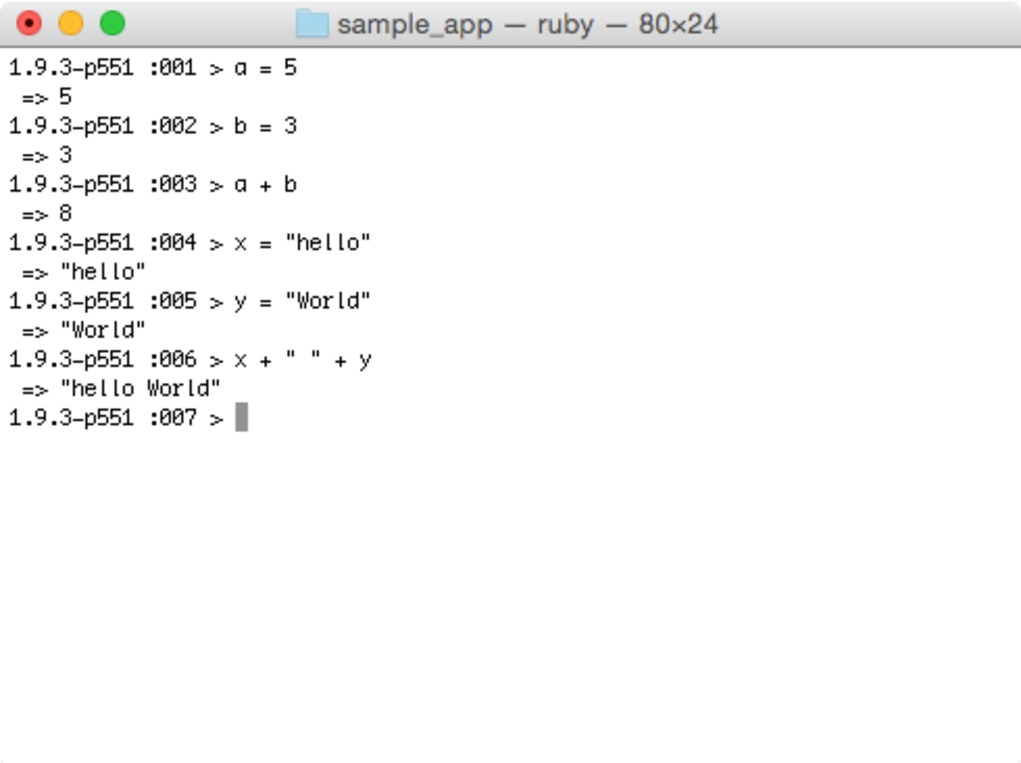
\includegraphics[width=150mm]{Bilder/Terminal.pdf}
    \caption{Terminalfenster unter Apple Mac OS X}  \label{Terminal}
  \end{center}
\end{figure}

Mit Hilfe des \textit{RoR}-Frameworks lassen sich dadurch schnell Web-Applikationen mit Datenbankbezug entwickeln, wobei der wesentlichen Vorteil in der Softwarearchitektur des Model-View-Controller-Paradigmas liegt.\footnote{Vgl. \cite{walter2008ruby}, S. 463} Das Paradigma besagt, dass eine durch einen Browser angestoßene Anfrage an den Server durch den \textit{RoR} \texttt{controller} verarbeitet wird. Der \texttt{controller} verarbeitet die Anfrage und leitet die nachfolgenden Schritte ein. Bei Web-Applikationen erfolgt eine solche Verarbeitung durch Anzeigen bzw. dem sogenannten \textit{Rendern} von HTLM-Dokumenten der \textit{RoR} \texttt{views} , die von Browsern angezeigt werden können. Der \texttt{controller} rendert die \texttt{views} und ermöglicht weitere \textit{RoR}-Befehle im HTML-Dokument. Bei komplexen und dynamischen Seiten übernimmt der \texttt{controller} geforderte Daten aus den \textit{RoR} \texttt{models}, die wiederum mit einer Datenbank verbunden sind. Durch diese Architektur lassen sind umfangreiche und an spezifische Anfragen angepasste Web-Applikationen entwickeln. Ein weiterer Vorteil von \textit{RoR} ist die einfache Implementierung von Unterprogrammen. Ein Unterprogramm ist in \textit{Ruby/RoR} ein \texttt{gem}, das durch den Bundler zur bestehenden Web-Applikation hinzugefügt wird und erweitert diese um weitere Konsolenbefehle.\footnote{Vgl. \cite{hartl2012ruby}, S. 9-17} Im nachfolgenden Kapitel wird die Entwicklung einer Web-Applikation mittels \textit{RoR} beschrieben. Dabei liegt die Besonderheit der Ausarbeitung auf die Beschreibung der Schnittstelle zwischen \textit{RoR} mit dem Programm \textit{GAMS}, damit das in diesem Kapitel vorgestellte Projektplanungsprobem gelöst werden kann, und der Integration eines notwendigen Unterprogramms (\texttt{gem}) zur Analyse der Daten des Projektplanungsproblems. Zusätzlich ist in dem Kapitel beschrieben, inwieweit ein weiteres Programm implementiert wird, damit die Projektplanung als Vorgangsknoten-Netzplan dargestellt werden kann.


\section{Implementierung des RCPSP mittels Ruby on Rails} \label{Haupt}
\subsection{Installation der Web-Applikation und der notwendigen Programme}
Die Applikation kann über nachfolgenden Terminalbefehl auf ein lokales Computerverzeichnis geklont werden.
\begin{lstlisting}[style=Befehl]
$ git clone https://github.com/rb4k/as-rcpsp.git
\end{lstlisting}
Zusätzlich zur Web-Applikation (inkl. \textit{RoR} in Version 1.9.3) müssen die Programme \textit{GAMS} zur Lösung von mathematischen Optimierungsmodellen und \textit{GraphViz} zur Visualisierung der Vorgangsbeziehungen auf dem lokalen Computerverzeichnis installiert sein. Die Programme können unter nachfolgenden Links bezogen werden:
\begin{itemize}
\item \textit{GAMS}: \texttt{http://www.gams.com/download/}
\item \textit{GraphViz}: \texttt{http://www.graphviz.org/Download\_windows.php}
\end{itemize}

\subsection{Darstellung der Funktionsweise der Anwendung anhand eines Guides für User}\label{User}
Die Funktionsweise der mit \textit{RoR} programmierten Anwendung \textit {\glqq Projektplanung\grqq} zur Lösung der Kapizitäts- und Kostenplanung des \textit{RCPSP} lässt sich am anschaulichsten mit Hilfe eines Userguides darstellen. 
Neben der Besonderheiten, die durch das Problem der Projektplanung auftreten, können im selben Zuge auch die Spezifika der einzelnen Benutzerrollen aufgezeigt werden. Beachtet werden muss, dass die hier vorgestellte Web-Applikation auf der Arbeit von \cite{hartl2012ruby} aufbaut.\\

Zunächst wird die Anwendung aus der Sicht eines Anwenders betrachtet, der sich nicht in die Applikation per Benutzererkennung eingeloggt hat. Konkret kann man sich darunter einen potentiellen Mitarbeiter des entsprechenden Projektes vorstellen, der sich über die Projektplanung informieren möchte, um sich gegebenenfalls als Mitarbeiter im Projekt (User) anzumelden. Im Testbetrieb wird der \textit{Ruby}-Server gestartet und durch Eingabe der URL \texttt{http://localhost:3000/} in die Adresszeile eines beliebigen modernen Browers wird die Startseite der Projektplanung angezeigt (siehe Abbildung \ref{Start}). Alternativ ist der Betrieb auf einem Webserver möglich, sofern die benötigte Software installiert und betriebsbereit ist. Auf der Startseite hat der User zum einen die Möglichkeit, sich anzumelden bzw. sich einzuloggen, für den Fall, dass er bereits User der Anwendung ist. \\

\begin{figure}[h!]
  \begin{center}
    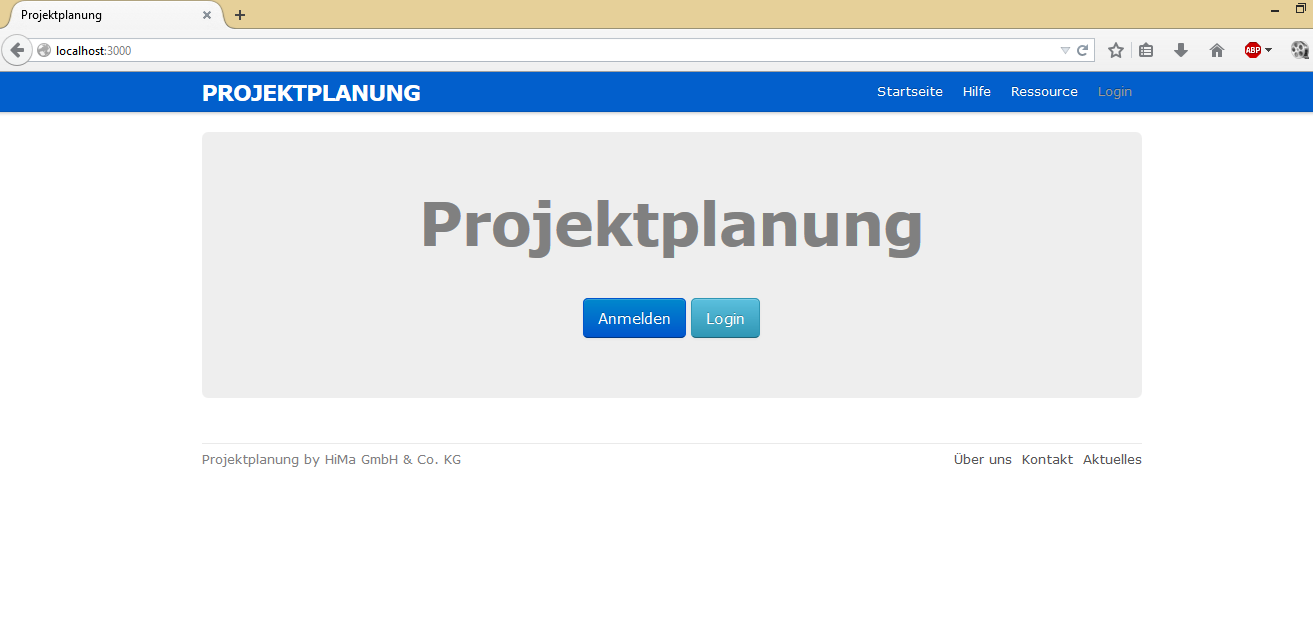
\includegraphics[width=150mm]{Bilder/Startseite_unsigned.png}
    \caption{Startseite Projektplanung Applikation}  \label{Start}
  \end{center}
\end{figure}

Bei der Startseite (\texttt{home.html.rb}) der RoR-Applikation handelt es sich um eine statische Seite (\texttt{static\_pages}) der \texttt{views}. Weiter gehören zu dieser Kategorie der HTML.RB-Dokumente die Seiten \texttt{about}, \texttt{contact}, \texttt{help} und \texttt{rcpsp}. Letztere wird zum späteren Zeitpunkt thematisiert. Ein Beispiel einer statischen Seite eines RoR \texttt{views} liefert Quellcode \ref{test} im Anhang \ref{rcodes}.\\

Anhand der \texttt{static\_pages} kann die Besonderheit von RoR deutlich gemacht werden. Durch das Model-View-Controller-Paradigma hilft der \texttt{static\_pages\_controller} bei der Verarbeitung von Anfragen. Es handelt sich hier um das typische Scaffolding (Bauprinzip) in \textit{RoR}, bei dem ein \texttt{controller}, \texttt{models} und \texttt{views} erstellt werden.\footnote{Vgl. \cite{walter2008ruby}, S. 464} Generiert werden können die Scaffolds durch  einen Ruby-Befehl im Terminalfenster.
\begin{lstlisting}[style=Befehl]
$ rails generate scaffold <name> <datenname:datentyp> 
\end{lstlisting}

Wie der Name aber schon andeutet, bedarf es bei den statischen Seiten kaum der Verarbeitung von Datensätzen der \textit{RoR} \texttt{models} zur Erstellung von dynamischen Seiten, wie der Quellcode \ref{spc} im Anhang \ref{rcodes} zeigt.\\

Für die \texttt{static\_pages} bedarf es einen speziellen \textit{Match}, der in der \texttt{config/routes.rb} Datei hinterlegt wird (Vgl. Quellcode \ref{routes}). Die \texttt{config/routes.rb} ordnet den Scaffolds und HMTL-Dokumente spezifische Verzeichnisse in der Applikation zu. RoR erkennt die Unterseiten der angelegten Scaffolds und ermöglicht die Verlinkung der Seiten auch ohne spezifische Angaben (Vgl. Quellcode \ref{routes} im Anhang \ref{rcodes}).\\

Mit dem Link \textit{Anmelden} erfolgt die Weiterleitung von der Startseite zur Anmeldeseite. Beschließt sich der Besucher der Seite, sich für das Projekt anzumelden, muss er alle Felder des Anmeldeformulars befüllen.

\begin{figure}[h!]
  \begin{center}
    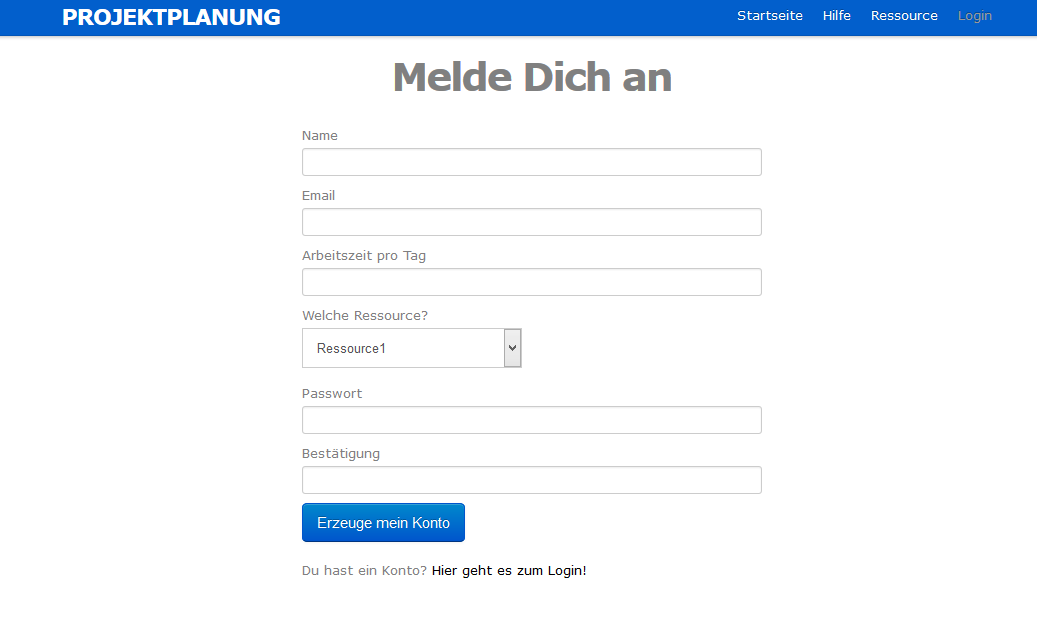
\includegraphics[width=120mm]{Bilder/Anmeldung.png}
    \caption{Anmeldebildschirm}  \label{Anm}
  \end{center}
\end{figure}

Neben dem Namen, einer Mailadresse und eines konformen Passwortes sind projektspezifische Informationen zur erfolgreichen Registrierung nötig. Im Feld \textit{Arbeitszeit pro Tag} muss ein entsprechender Wert eingegeben werden, den der neue User bereit ist, pro Tag für das Projekt an Zeit zu investieren. Wird in diesem Feld keine ganze Zahl, sondern eine Dezimalzahl oder ein Wort eingegeben, kann die Anmeldung im System nicht stattfinden. Es wird ein Fehler angezeigt, der das Defizit aufzeigt und behoben werden muss (siehe Abbildung \ref{Fehler}). Ausgelöst wird dieser Fehler durch einen Vermerk im zugehörigen RoR \texttt{models}, dass es sich um eine ganzahlilge Zahl handelt (\textit{Integer}). Der Quellcode \ref{fehler_code} im Anhang \ref{rcodes} zeigt dies anhand des hier betrachteten Beispiels.\\

\begin{figure}[h!]
  \begin{center}
    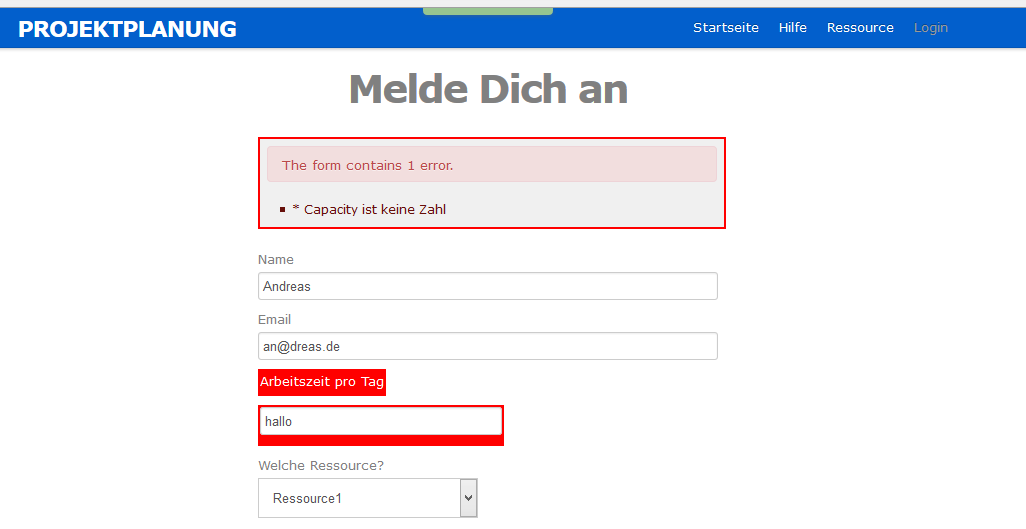
\includegraphics[width=120mm]{Bilder/Anmeldung_Fehleranzeige.png}
    \caption{Fehleranzeige bei der Anmeldung}  \label{Fehler}
  \end{center}
\end{figure}

Auf der Startseite (sowie allen anderen Seiten) sind neben Links wie \textit{Hilfe} und \textit{Kontakt} auch der Link zu \textit{Ressourcen}-Übersicht, in der alle Ressourcen des Projektes gelistet sind. Hier kommt der Grundsatz von RoR zum Tragen: \textit{Don’t repeat yourself}. Die Gestaltung und der Aufbau einer jeden Seite in der Web-Applikation orientiert sich anhand der CSS-Stylesheets bzw. der Layout-Dateien. Die Layout-Dateien sind unter \texttt{app/views/} gelistet und definieren auf jeder Seite spezifische Bereiche. Die \texttt{application.html.erb} generiert für jede Seite dieses einheitliche Layout, unterstützt durch die Dateien \texttt{\_footer.html.erb} und \texttt{\_header.html.erb}. Im \texttt{\_header.html.erb} ist der Link zur Ressourcen-Übersicht vermerkt (Vgl. Quellcode \ref{header} im Anhang \ref{header}).\\

Der \texttt{\_header.html.erb} zeigt einige \textit{If}-Befehle, mit denen unterschiedliche Daten anhand der Eigenschaften unangemeldeten, angemeldeten und Admin-Usern angezeigt werden. Durch Folgen des Links \textit{Ressource} wird die Index-Seite des \textit{RoR} \texttt{views/ressources} angezeigt (Siehe Abbildung ???). Der Quellcode \ref{index_res} im Anhang \ref{rcodes} zeigt die notwendige Programmierung für die Seite. \textit{RoR} durchläuft aufgrund der Aktivierung des Links die Aktion \textit{index} des dazugehörigen Controllers \texttt{resources\_controller.rb} und generiert die zugehörige HTML-Seite (\texttt{views}). Die Indexseite prüft, ob der aktuelle User angemeldet ist. Abhängig dieser Entscheidung integriert \text{RoR} unterschiedliche Seiteninhalte. Sofern der aktuelle User nicht angemeldet ist, wird eine vereinfachte Ressourcen-Übersicht angezeigt. In dieser Ansicht sind alle jeweilig aktuellen Ressourcen mit zugehörigen Namen aufgelistet, sowie dem Link \textit{Bewerben}, der wiederum mit der Anmeldeseite verlinkt ist.\\

Findet keine Anmeldung in die Web-Applikation statt, sind keine weiterführenden Tätigkeiten möglich. Die Startseite liefert keine weiterführenden Informationen und bei der Eingabe von anderen Links in die Adresszeile des Browers wird der aktuelle User zur \textit{Login}-Seite geführt, da alle Daten für nicht angemeldete Anwender gesperrt sind. %Die Verlinkung \textit{"http://localhost:3000/rcpsp/"} öffnet zwar die Seite der Projektplanung, alle angezeigten Buttons führen aber ebenfalls direkt zur Anmeldemaske. \\
Um die Applikation nutzen zu können, ist demzufolge die Anmeldung als User zwingend notwendig. Findet diese entweder nach erstmaliger Registrierung über den Link \textit{Anmelden} oder über \textit{Login} statt, wird die eigene Profilseite angezeigt (siehe Abbildung \ref{Profil}).\\

\begin{figure}[h!]
  \begin{center}
    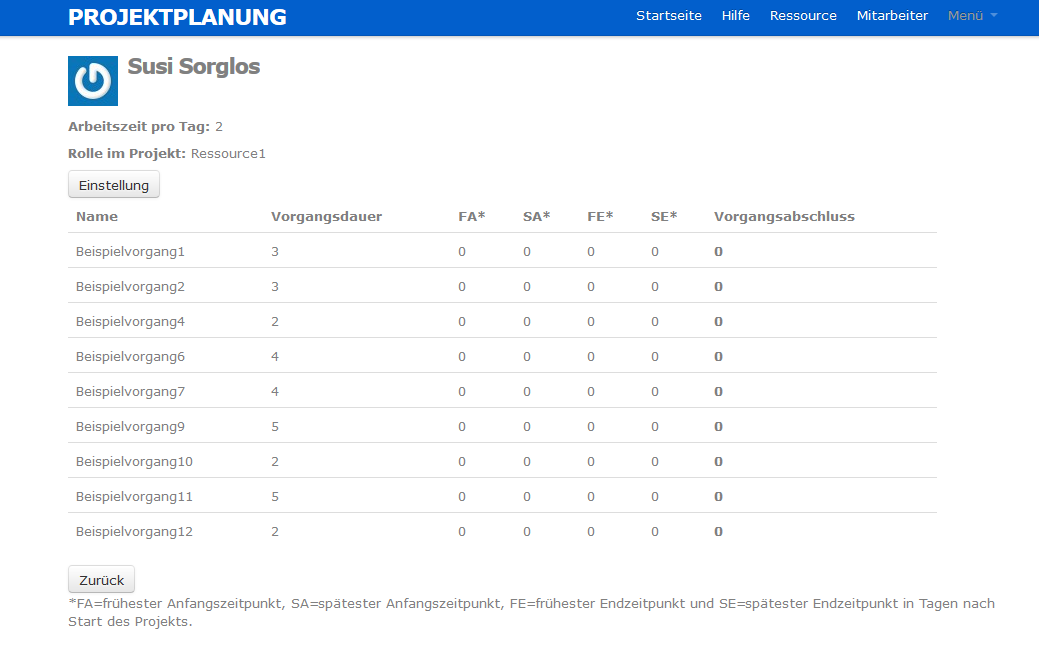
\includegraphics[width=120mm]{Bilder/Profilseite.png}
    \caption{Profilseite eines Users}  \label{Profil}
  \end{center}
\end{figure}

Die Profilseite gibt einen Überblick über all die Daten, die für den User in Hinblick auf das Projekt relevant sind. Es werden die Daten dargestellt, die bei der Anmeldung angegeben wurden (Arbeitszeit, Rolle im Projekt) sowie die Vorgänge, die durch die Wahl der Ressource für diesen User relevant sind, in denen er also arbeiten muss. Der Aufbau der Seite ist im Quellcode \ref{show_user} im Anhang \ref{rcodes} dargestellt.\\

Zu jedem Vorgang wird die Dauer und gegebenenfalls die Zeitspanne angegeben, wann er jeweils stattfindet. Die Grenze liegt zwischen dem frühesten Startzeitpunkt $FA_{i}$ und spätesten Endzeitpunkt $SE_{i}$ des Vorgangs $i$. Ebenfalls wird der kritische Pfad angezeigt. Dieser zeigt für die aufgeführten Vorgängen den Endzeitpunkt nach Start des Projekts unter Einhaltung der Ressourcenbeschränkung an, jeweils in Zeiteinheiten. Ob diese Tabelle mit Daten gefüllt ist, hängt davon ab, ob das Kapazitäts- bzw. Kostenplanungsproblem bereits gelöst wurde. Möchte der User seine Daten, wie z.B. die Wahl der Ressource oder die Quantität der Arbeitszeit, ändern, gelangt er über den Button \textit{Einstellung} zu einer Seite, die äquivalent aufgebaut ist wie die Anmeldeseite, um dort seine Daten zu aktualisieren. Nach korrekter Eingabe können die Daten über den Button \textit{Speichere Änderungen} gesichert werden. Auf der Profilseite erscheint daraufhin eine Anzeige \textit{Profil updated} mit der Bestätigung, dass das Profil aktualisiert wurde. Im Vergleich zum fremden Anwender gelangt der angemeldete User außerdem in der Kopfzeile über den Link \textit{Mitarbeiter} auf eine Übersicht aller Mitarbeiter, die für das Projekt auf dieser Applikation angemeldet sind. Die Profilseite jedes Mitarbeiters kann betrachtet werden mit all den Informationen, die auch auf der eigenen Profilseite einzusehen sind. Es können jedoch keine Änderungen vorgenommen werden. Neben der Verlinkung zu der Übersicht der Mitarbeiter lässt sich in der Kopfzeile ein Feld \textit{Menü} finden, dass die Unterpunkte \textit{Profil}, \textit{Einstellungen} und \textit{Logout} enthält. Die Verlinkung \textit{Profil} stellt eine Verlinkung zur Profilseite dar, unter \textit{Einstellungen} kann das eigene Profil aktualisiert werden.\\

Unter \textit{Ressourcen} kann der User, wie auch der nicht angemeldete Anwender, zur Übersicht der vorhandenen Ressourcen gelangen. Die Anzeige stellt sich für den angemeldeten User jedoch vielfältiger dar, als für den einfachen Anwender (siehe Abbildung \ref{ResUs}), da hier ein anderer Quellcode integriert ist (Vgl. Quellcode \ref{index_res}). Der Quellcode \ref{sign_res} im Anhang \ref{rcodes} zeigt den integrierten Inhalt.\\

\begin{figure}[h!]
  \begin{center}
    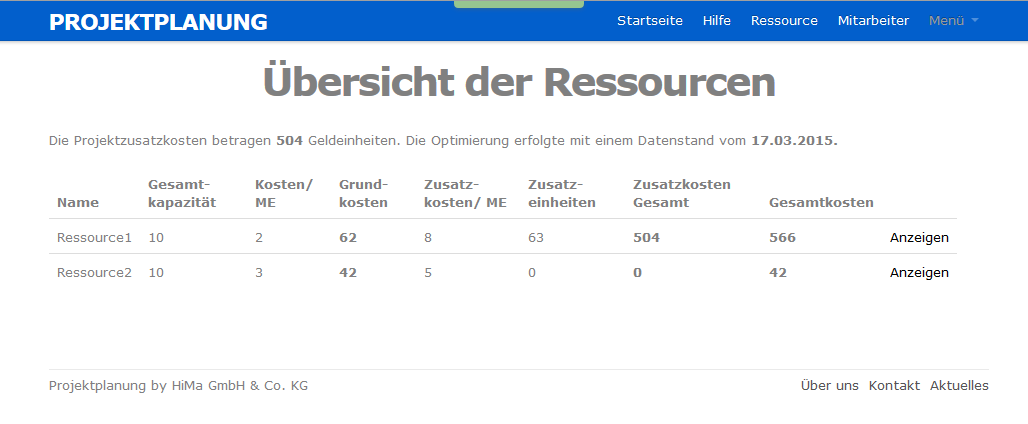
\includegraphics[width=120mm]{Bilder/Ressourcen_User.png}
    \caption{Übersicht der Ressourcen für User}  \label{ResUs}
  \end{center}
\end{figure}

Für den User sind alle Eigenschaften der verschiedenen Ressourcen einsehbar. Es werden die Gesamtkapazität, Kosten pro ME, Grundkosten und Zusatzkosten pro ME angezeigt. Wurde bereits eine Lösung für das Problem der Kostenplanung ermittelt, werden die kalkulierten Werte für die Zusatzeinheiten, gesamten Zusatzkosten und die Gesamtkosten pro Ressource dargestellt. Zudem wird der Zielfunktionswert, bei der Kostenplanung die gesamten anfallenden Zusatzkosten, in Verbindung mit dem Zeitpunkt der Optimierung über der Tabelle dargestellt. Die Darstellung der Tabellen in dieser Web-Applikation orientiert sich an dem Bootstrap-Framework\footnote{http://getbootstrap.com}. Alternativ bietet die App die Anzeige der Tabellen anhand einer JavaScript-Tabelle.\footnote{Auf Implementierung wurde jedoch aufgrund der möglichen Inkompatibilität zu bestimmten Browser und aufgrund der Laufzeitverbesserung der Web-Applikation verzichtet.} Über den Button \textit{Anzeigen} in der hier betrachteten Tabelle sind die Eigenschaften einer Ressource separat einsehbar. Da der User bzw. Mitarbeiter in diesem Modell durch die Planung innerhalb des Projektes eingeteilt wird und seine Rechte nicht über die Organisation der eigenen Daten hinaus reicht, hat er keine weiteren Kompetenzen bei der Nutzung dieser Applikation. \\

\subsection{Darstellung der Funktionsweise der Anwendung anhand eines Guides für Administratoren}\label{Admins}

Die Verwaltung der Mitarbeiter und die Organisation sowie Durchführung der Projektplanung kann ausschließlich nach der Anmeldung als Administrator (Admin) erfolgen. Der Admin gilt in dieser Anwendung als durchführende Gewalt. In dieser Testsituation ist \textit{Example User} mit den dafür notwendigen Berechtigungen ausgestattet. Alternativ lässt sich durch Änderung der booleschen Variable \texttt{admin = true} der Datenbank zum RoR \texttt{models/users} die Eigenschaft auch auf andere Datensätze (User) übertragen. Nach der erfolgreichen Anmeldung als User mit administrativen Rechten erscheint zunächst erneut die Profilseite, sofern die Anmeldung über die Startseite erfolgt. Im Gegensatz zu normalen Usern bietet die Seite eines Admins jedoch zusätzliche Handlungsspielräume neben der einfachen Auflistung der Vorgänge (siehe Abbildung \ref{ProAd}). Er hat die Möglichkeit, die Dauer der Vorgänge abzuändern oder Vorgänge aus dem Projekt zu löschen. Dies wird wieder über einen \textit{If}-Befehl gesteuert, wie der Quellcode \ref{show_user} aus dem Anhang \ref{rcodes} zeigt.\\

\begin{figure}[h!]
  \begin{center}
    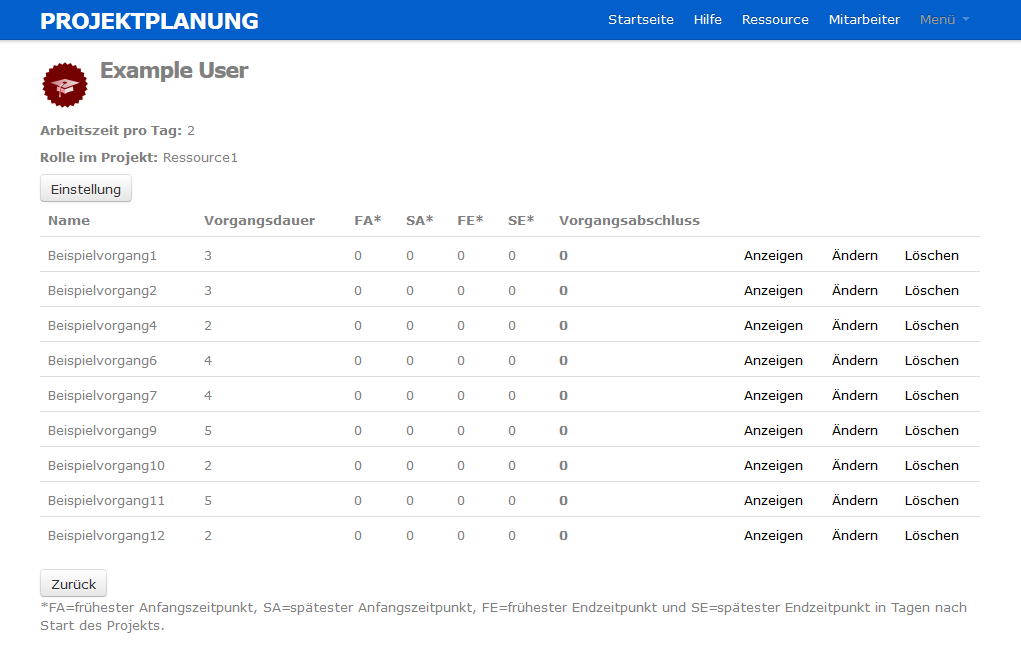
\includegraphics[width=120mm]{Bilder/Profilseite_Admin.png}
    \caption{Profilseite des Administrators}  \label{ProAd}
  \end{center}
\end{figure}       

In gleicher Weise stellt sich die Ausweitung der Kompetenzen bei den Ressourcen dar. Über die Auswahl des Links \textit{Ressourcen} im \textit{Header} existiert eine Verbindung zur Ressourcenübersicht. Dort können nun die Ressourcen ebenfalls gelöscht oder die Eigenschaften (Kosten und Zusatzkosten je ME) verändert werden. Des Weiteren kann über den Button \textit{Neue Ressource anlegen} eben dies vollzogen werden (Vgl. Quellcode \ref{index_res} im Anhang \ref{rcodes}).\\      

\begin{figure}[h!]
  \begin{center}
    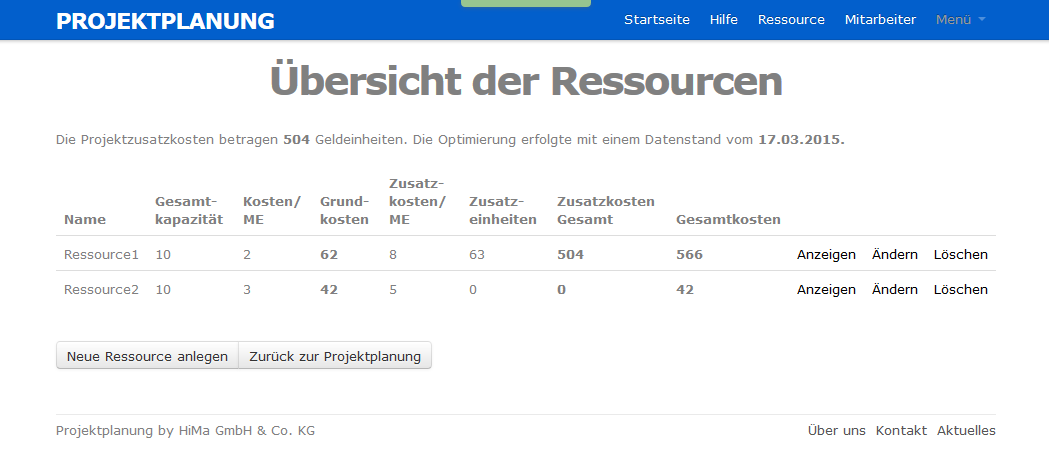
\includegraphics[width=120mm]{Bilder/Ressourcen_Admin.png}
    \caption{Übersicht der Ressourcen aus Sicht des Administrators}  \label{ResAd}
  \end{center}
\end{figure}     
  
Um nun zur Kernaufgabe der Applikation, der Projektplanung, zu gelangen, kann entweder der Button \textit{Zurück zur Projektplanung} auf der Seite zur Ressourcenübersicht getätigt werden, oder ausgehend von jeder beliebigen Seite der Web-Applikation in der Kopfzeile (\textit{Header}) unter \textit{Menü} der Unterpunkt \textit{Projektplanung} ausgewählt werden (siehe Abbildung \ref{RCPSP}). Bei dieser statischen Seite fließen Daten aus dem RoR \texttt{models/project} ein. Bei diesem Modell handelt es sich um eine Hilfsdatenbank ohne weiterer Beziehung zu anderen Modellen (Vgl. Abbildung \ref{schema} im Anhang \ref{db-schema}). Sie fungiert als Datenbank für unabhängige Parameter und hat damit nur einen Datensatz. Der Controller der statischen Seiten ruft über die Aktion \texttt{rcpsp} diesen Datensatz auf (Vgl. Quellcode \ref{spc} aus Anhang \ref{rcodes}). Dadurch kann das HTML.RB-Dokument \texttt{views/static\_pages/} den Datensatz aufgreifen und Formularfelder zur Eingabe der unabhängigen Parameter bereitstellen. Zu den unabhängigen Parametern dieses Formulars zählen die Datenfelder \texttt{path}, \texttt{startdate} und \texttt{deadline}, auf die im Verlauf der weiteren Beschreibung der Web-Applikation näher eingegangen wird.\\ %Wie bereits erwähnt, hat nur der Admin die Berechtigung, dieses Menü aufzurufen.


\begin{figure}[h!]
  \begin{center}
    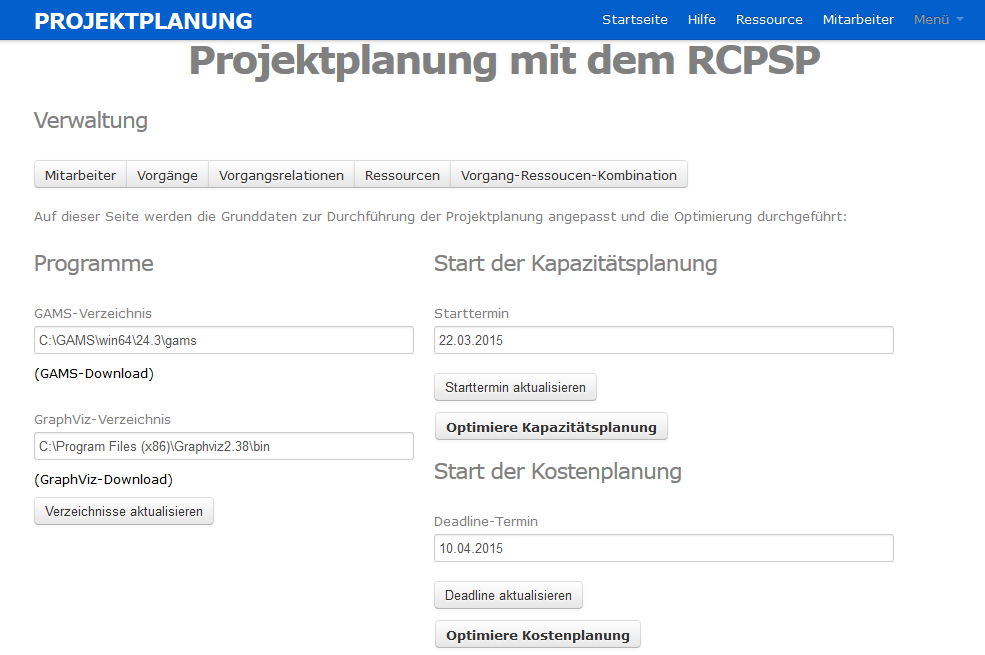
\includegraphics[width=120mm]{Bilder/Projektplanung.png}
    \caption{Projektplanung mit dem RCPSP - Übersicht}  \label{RCPSP}
  \end{center}
\end{figure}

Im oberen Bereich der Seite sind die Verlinkungen zur Verwaltung der nötigen Inputs zur Lösung beider Planungsproblematiken angesiedelt. Neben den bereits behandelten Links zu den Vorgängen und Ressourcen finden sich Verlinkungen zu den Vorgangsrelationen und Vorgang-Ressourcen-Kombinationen.\\ 

Die Übersicht der Relationen zwischen den Vorgängen stellt eine Auflistung eines jeden Vorgänger und Nachfolger dar. Durch anklicken auf den Button \textit{Graph anzeigen} wird die aktuelle Projektstruktur mittels Vorgangsknoten-Netzplan dargestellt (siehe Abbildung \ref{???}). Die genaue Implementierung dieses Graphen wird in Kapitel \ref{rgl-kapitel} beschrieben. Ein Admin kann eine Relationen löschen oder neue anlegen. Wenn er sich dazu entschließt, eine neue anzulegen, ist zu beachten, dass ein Strukturplan eines Projektes keine Zyklen beinhalten darf. Damit Zyklen verhindert werden, findet beim Prozess des Anlegens einer neuen Vorgangsrelation eine Prüfung statt. Beinhaltet die neu angelegte Relation einen Zyklus, tritt ein Fehler auf und die Relationen muss überarbeitet werden (siehe Abbildung \ref{VorErr}). So wird verhindert, dass der Strukturplan Zyklen enthält. Dieser Vorgang wird gesteuert durch die dafür zuständige Aktion \texttt{create} aus dem \textit{RoR} \texttt{procedure\_procedures\_controller} (Vgl. Quellcode \ref{ppc} im Anhang \ref{rcodes}). Inbegriffen in dieser Aktion ist ein frei-verfügbares Unterprogramm (\texttt{gem 'rgl'}\footnote{https://github.com/monora/rgl}). In Kapitel \ref{rgl-kapitel} wird die Integration und Funktionsweise dieses Unterprogramms beschrieben. \\

\begin{figure}[h!]
  \begin{center}
    
\includegraphics[width=120mm]{Bilder/Vorgangsrel_Fehler.png}
    \caption{Fehler aufgrund eines Zyklus in der topologischen Reihenfolge}  \label{VorErr}
  \end{center}
\end{figure}
 
Der Button \textit{Vorgang-Ressourcen-Kombination} führt zu eben dieser Übersicht. Neben der Auflistung können die Kombinationen verändert, gelöscht oder neu erstellt werden. Bei der Veränderung oder Erstellung ist zu beachten, dass die Angabe des Kapazitätsbedarfs nur mit Hilfe einer ganzen Zahl erfolgen darf. Entsprechend der Kapazitätsangabe bei der Bearbeitung eines Profils erscheint bei jeder anderen Art von Eingabe ein Fehler, der die Datenspeicherung verhindert (Vgl. Quellcode \ref{prm} im Anhang \ref{rcodes}).\\

Nachdem all diese Daten geprüft und gegebenenfalls verändert wurden, steht die Basis sowohl für die Optimierung der Kapazitäts- als auch der Kostenplanung. Bevor der Optimierungsprozess stattfinden kann, müssen noch einige Rahmenbedingungen geprüft werden. Da die Optimierung mit dem Programm \textit{GAMS} stattfindet, muss die Applikation auf dieses Programm zurückgreifen können. Dafür muss \textit{GAMS} auf dem hiesigen Computer installiert sein. Nach der Recherche des Installationsortes muss der korrekte Pfad in das dafür vorgesehene Feld der Übersichtsseite zur Projektplanung eingetragen werden, in dem der Beispielpfad zu sehen ist. Nach der Eingabe wird der Pfadzugriff durch \textit{Verzeichnis aktualisieren} in der Datenbank des RoR \texttt{models/project} gesichert (siehe Abbildung \ref{RCPSP}). Neben den Programmpfad muss ein Termin ausgewählt werden, zu dem das Projekt startet (siehe Abbildung \ref{Startdatum}). Anhand dieses Startdatums werden alle Daten bezüglich der Vorgänge berechnet, zudem stellt der Starttermin bei der Kostenplanung einen wichtigen Faktor dar. Durch die Betätigung des Feldes, das ein Muster anzeigt, öffnet sich ein Kalendermenü, in dem ein beliebiges Datum ausgewählt werden kann. Bei dem Datumsfeld handelt es sich ebenfalls um eine Applikationserweiterung (\texttt{Gem}) namens \glqq Bootstrap-Datepicker-Rails\grqq\footnote{https://github.com/Nerian/bootstrap-datepicker-rails} (Vgl. Quellcode \ref{gemfile} im Anhang \ref{rcodes}). Es handelt sich hier um ein Unterprogramm inkl. dazugehöriger JavaScrip-Datei. \\  

\begin{figure}[h!]
  \begin{center}
    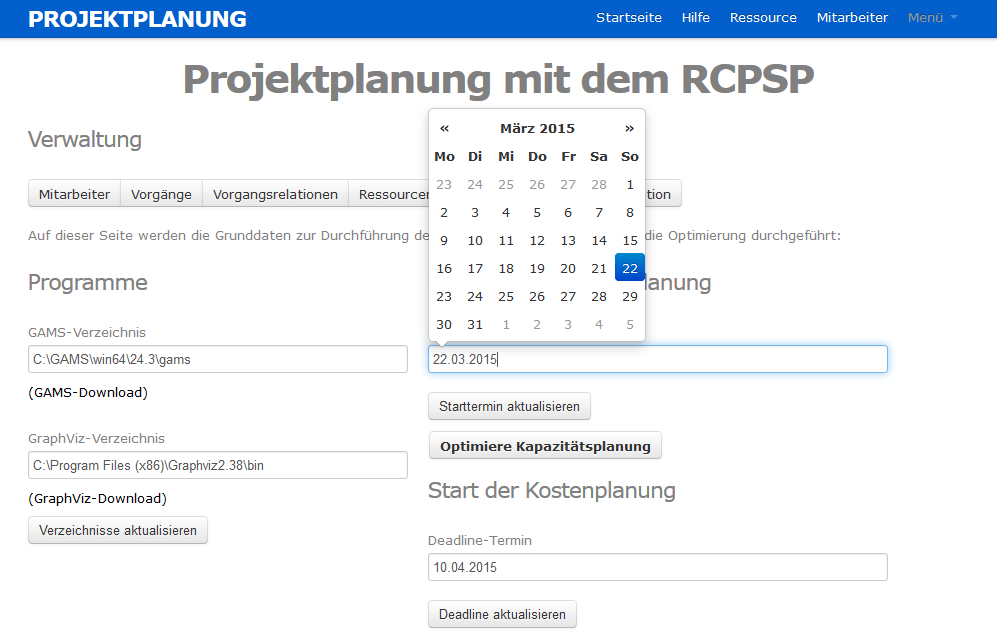
\includegraphics[width=120mm]{Bilder/Projektplanung_Datum.png}
    \caption{Einstellung des Starttermins anhand eines Kalendermenüs}  \label{Startdatum}
  \end{center}
\end{figure}

Nachdem das \textit{GAMS}-Verzeichnis und der Starttermin eingestellt wurden, kann die Kapazitätsplanung durch die Betätigung des Buttons \textit{Optimiere Kapazitätsplanung} durchgeführt werden. Es handelt sich hier um die Aktion \texttt{optimize} des RoR \texttt{rcpsps\_controller} (Vgl. Quellcode \ref{rcpspc} im Anhang \ref{rcodes}). Die Aktion dient dazu, die Include-Dateien für die \textit{GAMS}-Optimierung zu schreiben und eben diese durch Aufrufen der \textit{GAMS}-Software zu starten. Bei der \textit{GAMS}-Optimierung handelt es sich um die Datei mit dem Quellcode \ref{rcpsp1} aus Anhang \ref{Imp}. Nach einer Rechenzeit, währenddessen der Button, mit dem die Optimierung gestartet wurde, auf den Rechenprozess hinweist, leitet die Applikation den Admin direkt zu der Übersicht der Vorgänge. Dieser Schritt wird durch die Hilfsaktion \texttt{solution} des RoR \texttt{rcpsps\_controller} unterstützt, die parallel aufgerufen wird. Nachdem die \textit{GAMS}-Optimierung vollzogen ist, liest der RoR \texttt{rcpsps\_controller} die von der \textit{GAMS}-Optimierung erstellten Text-Dateien ein und schreibt diese direkt in die dafür vorgesehen Datenbank. Bei der Kapazitätsplanung wird hauptsächlich die Datenbank des RoR \texttt{models/procedure} angesprochen. Wie bereits in Abbildung \ref{ProAd} dargestellt, sind in der Übersicht der Vorgänge alle möglichen Zeitpunkte dargestellt, an denen die einzelnen Vorgänge stattfinden können. Zusätzlich wird die Projektdauer über der Tabelle und der kritische Pfad, durch den die Projektdauer erzielt wird, in die Tabelle geschrieben (siehe Abbildung \ref{Kap}).\\
\begin{figure}[h!]
  \begin{center}
    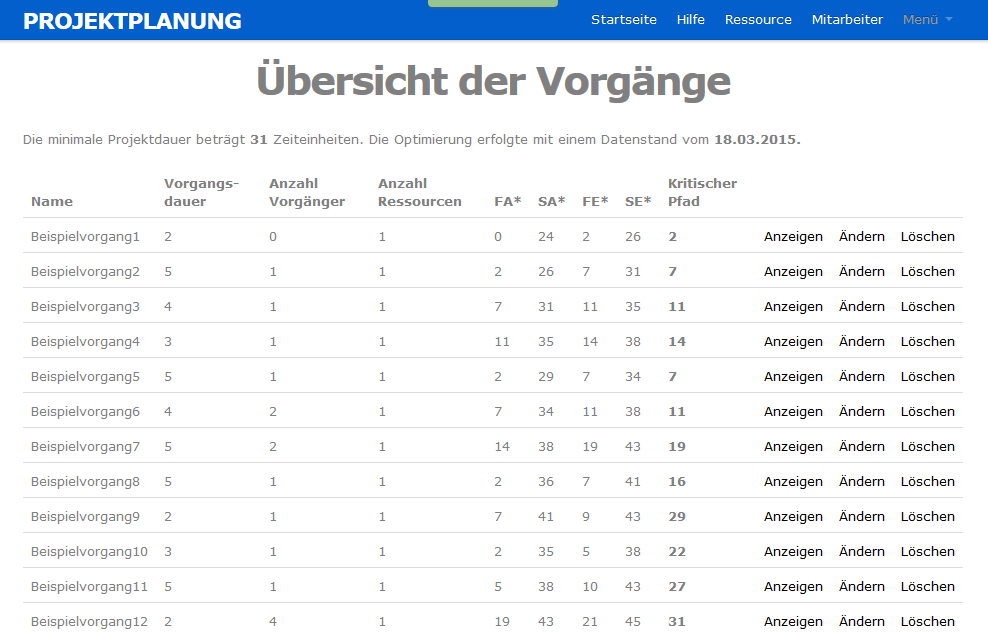
\includegraphics[width=120mm]{Bilder/Kapazitaetsplanung.png}
    \caption{Ergebnis der Kapazitätsplanung}  \label{Kap}
  \end{center}
\end{figure}

Die Besonderheit der Aktion \texttt{optimize} ist, dass \textit{RoR} die durch die \textit{GAMS}-Optimierung (Quellcode \ref{rcpsp2} aus Anhang \ref{Imp}) erstellte Textdatei zum Parameter $X_{it}$ trotz der zwei Indizes auslesen kann. Dies erfolgt durch einen \textit{If}-Befehl, wie der Ausschnitt (Quellcode \ref{rcpsp_a}) des Quellcodes \ref{rcpspc} aus dem Anhang \ref{rcodes} zeigt. Die Kapazitätsplanung ist mit dem Einlesen der Ergebnisse abgeschlossen.\\

\lstinputlisting[language=ruby, firstline=104, lastline=116, caption=Ausschnitt aus dem RoR-Controller für das RCPSP, style=Listing, label= rcpsp_a]{/Users/Superuser/as-rcpsp/app/controllers/rcpsps_controller.rb}

Über den Button \textit{Zurück zur Projektplanung} gelangt ein Admin zurück zur Verwaltungsseite. Sofern die Kostenplanung gewünscht ist, kann diese über die Verwaltungsseite gestartet werden. Bevor der optimale Kostenplan für das vorhandene Projekt berechnet werden kann, muss zunächst äquivalent zur Einstellung des Starttermins eine Deadline eingerichtet werden. Dies funktioniert erneut über ein Kalendermenü des \glqq Bootstrap-Datepicker-Rails\grqq. Es sollte bei der Bestimmung der Deadline darauf geachtet werden, dass die Deadline in einem sinnvollen Verhältnis zum Starttermin steht. Eine zu kurze oder lange Zeitspanne zwischen den beiden Terminen kann zu unbrauchbaren Ergebnissen führen. Wurde eine geeignete Deadline ausgewählt und die Optimierung des Kostenplans gestartet, öffnet sich nach einer kurzen Rechenzeit die Übersicht der Ressourcen. Dieses erfolgt mit der Aktion \texttt{optimize2} und \texttt{solution2} des \texttt{rcpsps\_controller}.\\ 

Auf der Seite mit der Ressourcenübersicht sind die Projektkosten und die Zusatzkosten, die jede Ressource durch Einhaltung der Deadline verursachen, ausgelesen (siehe Abbildung \ref{ResAd}). Bei der Kostenplanung ist jedoch nicht nur relevant, wie hoch die Kosten zur Durchführung des Projektes sind, sondern auch die Zeitpunkte, zu denen die Vorgänge stattfinden. Um dies zu untersuchen, bietet sich dem Admin die Möglichkeit, ein weiteres Mal die Seite mit der Übersicht der Vorgänge aufzurufen. Auf dieser Seite sind die frühesten und spätesten Zeitpunkte sowie der Abschluss jedes Vorgangs unter Einhaltung der Ressourcenbeschränkung in die Tabelle eingelesen. Die alten Ergebnisse der Kapazitätsplanung sind gelöscht, damit kein veralteter Wert angezeigt wird (siehe Abbildung \ref{VorKo}). Somit sind alle Informationen des Kostenplans einsehbar, die Kostenplanung ist ebenfalls abgeschlossen.\\  

\begin{figure}[h!]
  \begin{center}
    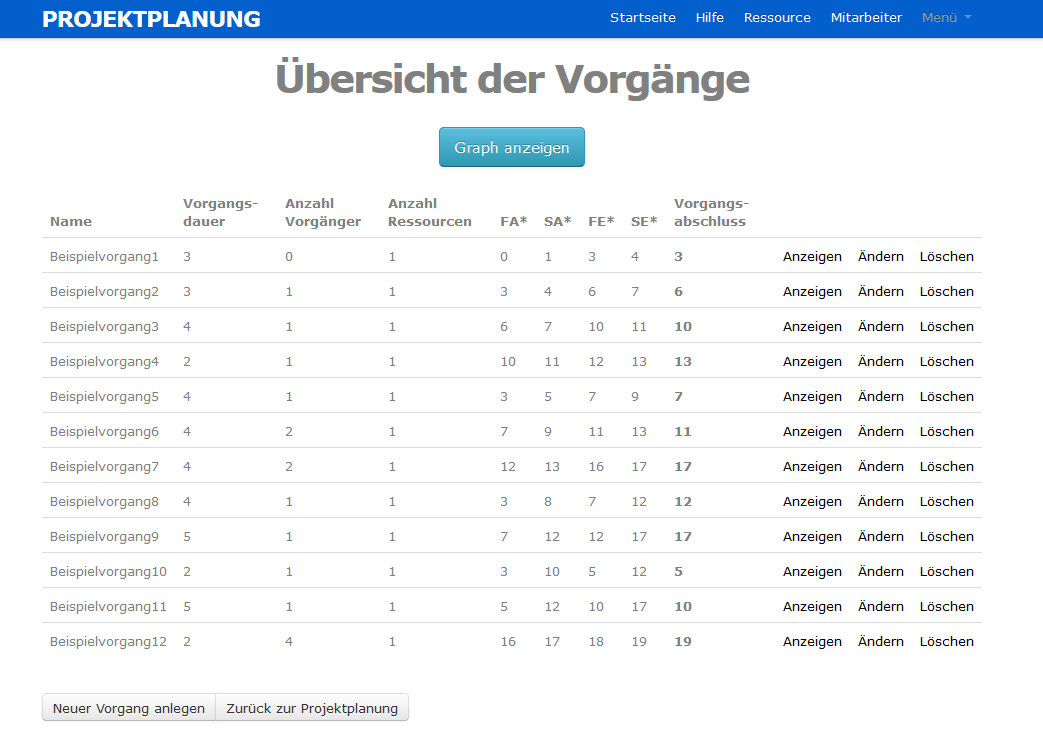
\includegraphics[width=120mm]{Bilder/Vorgaenge_Kostenpl.png}
    \caption{Ergebnis der Kostenplanung}  \label{VorKo}
  \end{center}
\end{figure}

\subsection{Integration des Unterprogramms \textit{\glqq rgl\grqq} und des Programms \textit{GraphViz} in die Web-Applikation}\label{rgl-kapitel}
Für die Lösung des Projektplanungsproblems bedarf es der topologischen Reihenfolgebeziehung der einzelnen Vorgänge untereinander. Weiter dürfen keine Zyklen in der Projektstruktur inbegriffen sein.\footnote{????} Zur Prüfung der aktuellen Projektstruktur der aktuell gespeicherten Datensätze zu dem Projekt (Vorgänge und Vorgangsrelationen) muss \textit{RoR} ein Algorithmus hinterlegt werden, der die Projektstruktur nach Zyklen untersucht. Eine Sammlung von hierfür geeigneten Algorithmen bietet die Ruby Graph Library (RGL) in Form des Unterprogramms \texttt{gem 'rgl'}\footnote{https://github.com/monora/rgl}. Mit dieser \texttt{gem} wird die Web-Applikation um die dafür notwendigen Kommandobefehlen erweitert. Bei der \texttt{gem 'rgl'} handelt es sich um eine Sammlung von Kommandobefehlen für die Graphentheorie, deren Datenstruktur und die zur Analyse notwendigen Algorithmen. Alternativ gibt es andere Sammlungen bzw. Erweiterungen der \texttt{gem 'rgl'}, wie z. B. die \texttt{gem 'plexus'}.\\

In der hier betrachteten Web-Applikation zur Lösung des Projektplanungsproblems ist die \texttt{gem 'rgl'} implementiert. Eine bestehende Web-Applikation kann durch eine \texttt{gem} mittels \textit{GitHub} und dazugehörigem Terminalbefehl erweitert werden. Beachtet werden muss jedoch, dass in der \texttt{Gemfile}, in der \texttt{Rakefile} sowie in ggf. anderen Dateien Fehler durch den \texttt{pull}-Befehl auftreten könnten. Daher empfiehlt es sich einen neuen \texttt{git branch} zu erstellen. Nachfolgende Kommandobefehle im Terminal zeigen die vorher beschriebenen Schritte:  
\begin{lstlisting}[style=Befehl]
$ cd <Verzeichnis der Web-Applikation>
$ git branch -b <Branch-Name>
$ git pull https://github.com/monora/rgl.git
\end{lstlisting}

Nach dem das Verzeichnis der Web-Applikation um die Dateien der \texttt{gem 'rgl'} erweitert ist, muss in der \texttt{Gemfile} das nötige \texttt{gem} aktiviert werden (siehe Ausschnitt aus Quellcode \ref{gemfile}).

%%%%%%GEMFILIE
\lstinputlisting[language=ruby, firstline=11, lastline=15, caption=Ausschnitt der Gemfile der Web-Applikation Projektplanung, style=Listing, label=gemfile1]{/Users/Superuser/as-rcpsp/Gemfile}

Durch den Befehl zur Installation mittels \textit{Bundler} wird die Web-Applikation um die ergänzten \texttt{gem}-Dateien erweitert. 
\begin{lstlisting}[style=Befehl]
$ bundle install
\end{lstlisting}

Damit sind neue Kommandobefehle innerhalb der Programmierung der Web-Applikation möglich. Zur Prüfung der Projektstruktur auf Zyklen wird der Algorithmus bzw. die \textit{Klasse} \texttt{RGL::TopsortIterator} der \texttt{gem 'rgl'} verwendet.\footnote{http://www.rubydoc.info/github/monora/rgl/RGL/TopsortIterator} Die \textit{Klasse} ordnet die Datensätze der Vorgangsbeziehung in eine lineare Ordnung ein. Anschließend wird der dadurch generierte Graph nach Zyklen durchsucht. Abbildung \ref{rgl-vonseite} zeigt dies anhand eines Beispiels.
\begin{lstlisting}[caption=Prüfung auf Zyklen mittels des Unterprogramms \glqq rgl\grqq, style=Listing, label=rgl-vonseite]
>> require 'rgl/adjacency'
>> dg=RGL::DirectedAdjacencyGraph[1,2 ,2,3 ,2,4, 4,5, 6,4, 1,6]
(1-2)(1-6)(2-3)(2-4)(4-5)(6-4)
>> require 'rgl/topsort'
>> dg.acyclic?
true
\end{lstlisting}

Für die hier betrachtete Web-Applikation bedarf es eines Zugriffs auf das Datenbankmodell des RoR \texttt{models/procedure\_procedure.rb} zur Prüfung der Projektstruktur. Das Modell dient dazu die einzelnen Vorgänge in eine Beziehung zueinander zu bringen, damit in der \textit{GAMS}-Optimierung die topologische Reihenfolge eingehalten werden kann. Das Modell hilft aber auch zur Generierung eines Graphs für das Unterprogramm \texttt{rgl}. Dafür wird eine Schleife erstellt, in der die Vorgänger (\texttt{prepro\_id}) und die Nachfolger (\texttt{sucpro\_id}) eines jeden Vorgangs (\texttt{procedure}) in einen direkten Nachbarschaftsgraphen ergänzt werden (siehe Quellcode \ref{rgl-vonseite}).

\begin{lstlisting}[caption=Erstellung eines Graphen mittels des Unterprogramms \glqq rgl\grqq, style=Listing, label=rgl-vonseite]
require 'rgl/adjacency'
result = RGL::DirectedAdjacencyGraph.new ProcedureProcedure.all.each { | x |
result.add_edge x.prepro_id , x.sucpro_id }
\end{lstlisting}

Nachdem dieser Graph generiert ist, wird dieser durch die Methode \texttt{\#acyclic?}\footnote{http://www.rubydoc.info/github/monora/rgl/RGL/Graph\#acyclic\%3F-instance\_method} auf bestehende Zyklen untersucht. Diese Untersuchung ist in dem \textit{RoR} \texttt{controller} unter der Aktion \texttt{create} ergänzt. Abbildung \ref{vorgangsbez} zeigt einen Ausschnitt mit der hier beschriebenen Aktion.
\lstinputlisting[language=ruby, firstline=38, lastline=59, caption=Ausschnitt aus dem RoR-Controller für die Vorgangsbeziehungen, style=Listing, label=vorgangsbez]{/Users/Superuser/as-rcpsp/app/controllers/procedure_procedures_controller.rb}

Weiter bietet das Unterprogramm \texttt{rgl} die Möglichkeit, eine \texttt{dot}-Datei zu erstellen, damit der Graph mittels des Programms \textit{GraphViz} visualisiert wird.
\begin{lstlisting}[caption=Prüfung auf Zyklen mittels des Unterprogramms \glqq rgl\grqq, style=Listing, label=rgl-vonseite]
>> require 'rgl/adjacency'
>> dg=RGL::DirectedAdjacencyGraph[1,2 ,2,3 ,2,4, 4,5, 6,4, 1,6]
>> require 'rgl/dot'
>> dg.write_to_graphic_file
"graph.dot"
\end{lstlisting}

Zur Visualisierung der \texttt{dot}-Datei bedarf es jedoch der Integration des Open-Source-Programms \textit{GraphViz} in die Web-Applikation. Mit dem Programm ist es möglich Strukturinformationen als abstrakte Graphen und Netzwerke darzustellen.\footnote{http://www.graphviz.org/About.php} Damit \textit{RoR} mit dem Programm kommunizieren kann, wird seitens der Anbieter empfohlen das Unterprogramm \texttt{gem 'ruby-graphviz'} zu verwenden. Nachdem die Installation des Unterprogramms durchgeführt und das Programm \textit{GraphViz} in einem lokalen Computerverzeichnis gespeichert ist, kann die \texttt{dot}-Datei mittels Kommandobefehl ausgelesen und visualisiert werden. Dies erfolgt im RoR \texttt{controllers/procedure\_procedures\_controller.rb} sowie auf der Unterseite \texttt{graph.html.rb} der \textit{RoR} \texttt{views/procedure\_procedures} (Vgl. Quellcode \ref{ppc} bzw. \ref{graphv} im Anhang \ref{rcodes}). Abbildung \ref{defgraph} zeigt die Aktion zur Erstellung des Graphen.
\lstinputlisting[language=ruby, firstline=6, lastline=17, caption=Ausschnitt des RoR-Controller für die Vorgangsrelationen, style=Listing, label=defgraph]{/Users/Superuser/as-rcpsp/app/controllers/procedure_procedures_controller.rb}


\section{Kritische Würdigung des Anwendungssystems} \label{krit}
%Die kritische Betrachtung impliziert neben den Besonderheiten des Programms auch die zukünftigen Verbesserungsmöglichkeiten dieses Anwendungssystems.
Die hier implementierte Applikation behandelt ausschließlich das \textit{RCPSP} bei exakt einem vorhandenen Projekt. Die Multiprojektplanung wurde außer Acht gelassen. Mit der Einführung der Multiprojektplanung eröffnen sich zwar neue Problemstellungen bei der Implementierung, es bietet jedoch auch neue Anwendungsmöglichkeiten der Applikation. Anstatt einzelne Aspekte eines Projektes zu optimieren, kann nun ein Portfolio an mehreren Projekten erstellt werden. Ein Mitarbeiter hat somit die Wahl, an welchen Projekten er partizipieren möchte und die Durchführung des Projektportfolios ist Ziel der Optimierung. Es findet dementsprechend eine Projektion der Kapazitäts- und Kostenplanung auf die Multiprojektplanung statt.\\

Die tatsächlich durchgeführte Programmierung bietet ebenfalls Verbesserungspotential. Auf der Übersichtsseite der Projektplanung, auf der die Optimierungsvorgänge gestartet werden können, finden sich auch die Felder zur Aktualisierung des Starttermins und der Deadline. Die Felder und Funktionen, die in diesem Zusammenhang ausgelöst werden, funktionieren zwar fehlerfrei, die zeitliche Abhängigkeit ist aber nicht in der Form gegeben, wie es die Bezeichnungen voraussetzen. Wird die zeitliche Reihenfolge vertauscht, führt das Modell die Optimierung fehlerhaft durch. Der Termin der Deadline muss laut der implementierten Regularien zeitlich nachfolgend zum Starttermin stattfinden. \\

Ein weiteres Problem tritt bei der Aktualisierung der Pfade für die Programme \textit{GAMS} und \textit{GraphViz} auf (siehe Abbildung \ref{RCPSP}). Die Lösung aller Planungsprobleme erfolgt erst nach der Angabe des korrekten Pfads von \textit{GAMS}. Nach diesem Schema funktioniert die Erstellung des Graphen der Vorgangsrelationen nur, wenn erfolgreich auf \textit{Graphviz} zurückgegriffen werden kann. Diese Kausalitäten führen zu der Frage, was bei der Angabe von falschen Pfaden für das jeweilige Programm passiert. Faktisch funktionieren sie nicht. Beim Start der Optimierung mit einem falschen \textit{GAMS}-Pfad sucht der Controller vergeblich nach \textit{GAMS}. Statt den Vorgang abzubrechen, bleibt der \textit{Ruby}-Server an dieser Stelle hängen und der Nutzer kann keine weiteren Aktionen ausführen. Um dieses \glqq Abstürzen\grqq\; des Servers zu verhindern, falls der Programmpfad inkorrekt ist, könnte ein \textit{Timeout}-Befehl die Aktion nach einer vorgegebenen Zeitspanne abbrechen. So wäre es möglich, den Pfad zu ändern und den Vorgang erneut zu starten. Die Aktion \textit{Timeout} ist dem Framework \textit{RoR} inbegriffen. Eine andere Möglichkeit als die Aktion \textit{Timeout} ist das Unterprogramm \textit{\glqq Terminator\grqq}. \textit{\glqq Terminator\grqq} ist keine interne \textit{RoR}-Methode, daher muss der passende \texttt{gem} installiert werden, damit \textit{RoR} diese Methode verwenden kann.\footnote{https://github.com/ahoward/terminator}\\

Auch bei der Verwaltung der Vorgänge und Vorgangsrelationen offenbaren sich Lücken, die in späteren Ausarbeitungen überarbeitet werden sollten. Das Anlegen, Ändern und Löschen von Vorgängen funktioniert reibungslos. Zur Darstellung der Vorgangsrelationen wird das Programm \textit{GraphViz} verwendet, unter Zuhilfenahme des Unterprogramms \texttt{gem 'ruby-graphviz'}. Der Programmcode dieses Unterprogramms ist übernommen, nur eine Anwendung des Unterprogramms an die Gegebenheiten der Problemstellung findet statt. Diese Datenübernahme hat zur Folge, dass der Name jedes Vorgangs aus \textbf{mindestens zwölf Zeichen} bestehen muss. Bei einem kürzeren Vorgangsnamen zeichnet das Programm keinen Graphen. Die Gründe dafür konnten in dieser Arbeit nicht abschließend geklärt werden, da der gesamte Programmcode des Unterprogramms und des Programms \textit{GraphViz} in der kurzen Zeit der Erstellung dieser Arbeit nicht vollständig untersucht werden konnte. Daher ist in dieser Arbeit eine Mindestlänge für den Namen eines Vorgangs vorgegeben. Das ursprüngliche Problem von \textit{GraphViz} besteht dadurch weiterhin. Auf andere Funktionen der Vorgänge oder Vorgangsrelationen hat dieser Umstand keinen Einfluss. Die Vorgangsrelationen stellen einen wichtigen Part der Projektplanung dar. Schließlich ist die Bestimmung der Reihenfolge der abzuarbeitenden Vorgänge die Basis für viele andere Operationen auf dem Weg zur Projektopimierung. Beim Anlegen einer neuen Vorgangsrelation dürfen, wie bereits beschrieben, keine Zyklen entstehen. Es findet aber keine Prüfung statt, ob die neu angelegte Vorgangsrelation bereits existiert. Folglich wird nicht verhindert, dass z.B. die Relation von \textit{Vorgang 1} zu \textit{Vorgang 2} zwei Mal angelegt wird. Für alle weiteren Prozesse resultieren keine Schäden, da doppelt vorhandene Relationen nicht beachtet werden, trotzdem handelt es sich hier um eine Prüfungslücke im Modell der Vorgangsrelationen. Diese Problematik der Möglichkeit von inhaltlich identischen Datensätze betrifft jedes Datenmodell.\\      
  
\section{Fazit} \label{Fazit}
In dieser Ausarbeitung sind zunächst die Problematiken der Projektplanung dargelegt sowie das \textit{RCPSP} für die Kapazitäts- und Kostenplanung formuliert. Dabei steht neben der Lösung des Modells mit einem Programm für mathematische Modellformulierungen auch die Integration sowie Verknüpfung mit einer Web-Applikation im Vordergrund. Ziel ist es, eine Web-Applikation zu erstellen, die im Hintergrund der Anwendung auf das Lösungstool, dass die Rechnungen durchführt, zurückgreift, die Ergebnisse abruft und darstellt.\\

Das \textit{RCPSP} wird in dem Programm \textit{GAMS} für mathematische Optimierungsprobleme formuliert und mit dessen Hilfe wird die LP-Relaxation gelöst. Da der Schwerpunkt dieser Arbeit auf dem Framework \textit{RoR} liegt, sind in der\textit{GAMS}-Modellformulierung nur die essentiellen Bestandteile zur Lösung des \textit{RCPSP} implementiert. Dank einer Schnittstelle zwischen dem Framework \textit{RoR} und dem Programm \textit{GAMS} ist es möglich, einen Großteil der Daten in \textit{RoR}-Programmiersprache zu formulieren, um diese dann in \textit{GAMS} einlesen zu lassen. Der Schwerpunkt liegt dementsprechend auf der Implementierung in \textit{RoR} und der Bildung der Schnittstelle.\\

Bei der Erstellung der Applikation ist die herausragende Rolle der Controller zu erwähnen. %Ein Controller ist für jede Art von Programmierungselement erforderlich, sofern ein Datenmodell mit einbezogen wird. %, unabhängig von der Tatsache, ob es sich zum Beispiel um die Entwicklung eines Datenmodells oder die Strukturierung der Homepage handelt.
In den jeweiligen Controllern werden alle dynamischen Aktionen definiert, auf die in anderen Verzeichnissen oder Datenmodellen zurückgegriffen werden. Nur Aktionen, die im Controller hinterlegt sind, können in der HTML-Darstellung der Seite aufgerufen bzw. genutzt werden. Alternativ wird der Controller für die Schnittstelle zu \textit{GAMS} oder \textit{GraphViz} benötigt. Falls der Controller fehlerhaft programmiert ist, führt dies zwangsläufig an einem gewissen Punkt der Applikation zu Komplikationen. Am Beispiel des \textit{RCPSP}-Controller (Quellcode \ref{rcpspc} im Anhang \ref{rcodes}) lässt sich die Signifikanz des Controllers in \textit{RoR} demonstrieren.\\

Im \textit{RCPSP}-Controller sind alle Aktionen bezüglich der Optimierung der Kapazitäts- und Kostenplanung hinterlegt. Die Aktion \texttt{optimize} beinhaltet alle Schritte, die \textit{RoR} durchführen muss, damit die \textit{GAMS}-Datei zur Lösung der Kapazitätsplanung den vollständigen Input erhält, das System gestartet sowie der Output korrekt ausgelesen wird. Die durch das Betätigen des Buttons \textit{Optimiere Kapazitätsplanung} ausgelöste Aktion \texttt{optimize} (siehe Abbildung \ref{RCPSP}), funktioniert ausschließlich durch die korrekte Programmierung des Controllers.\\   

Schließlich liefert die Arbeit eine umfangreiche Darstellung der Web-Applikation für die Projektplanung mittels \textit{RoR}, \textit{GAMS} und \textit{GraphViz}. Dabei wird auf die Besonderheiten der Programmierung eingegangen und explizit auf die Integration weiterer Unterprogramme in dem Framework \textit{RoR}.


\bibliographystyle{Prod_Seminar}    %legt die zu verwendende BIBTEX-Stildatei fest
\newpage
\bibliography{Literatur}    %an der Stelle zu verwenden, an der das Literaturverzeichnis gesetzt werden soll;
                            %Literatur ist der Dateiname der BIB-Datei mit den LiteraturLiteratur-Informationen

\newpage
%%%%%%%%%%%%%%%%%%%%%%%%%%%%%%%%%%%%%%%%%%%%%%%%%%%%%%
%
%    ggf. Anhang
%
%%%%%%%%%%%%%%%%%%%%%%%%%%%%%%%%%%%%%%%%%%%%%%%%%%%%%%
\begin{appendix}
\section{Anhang}

\subsection{Datenbankschema}\label{db-schema}

\begin{figure}[h!]
  \begin{center}
    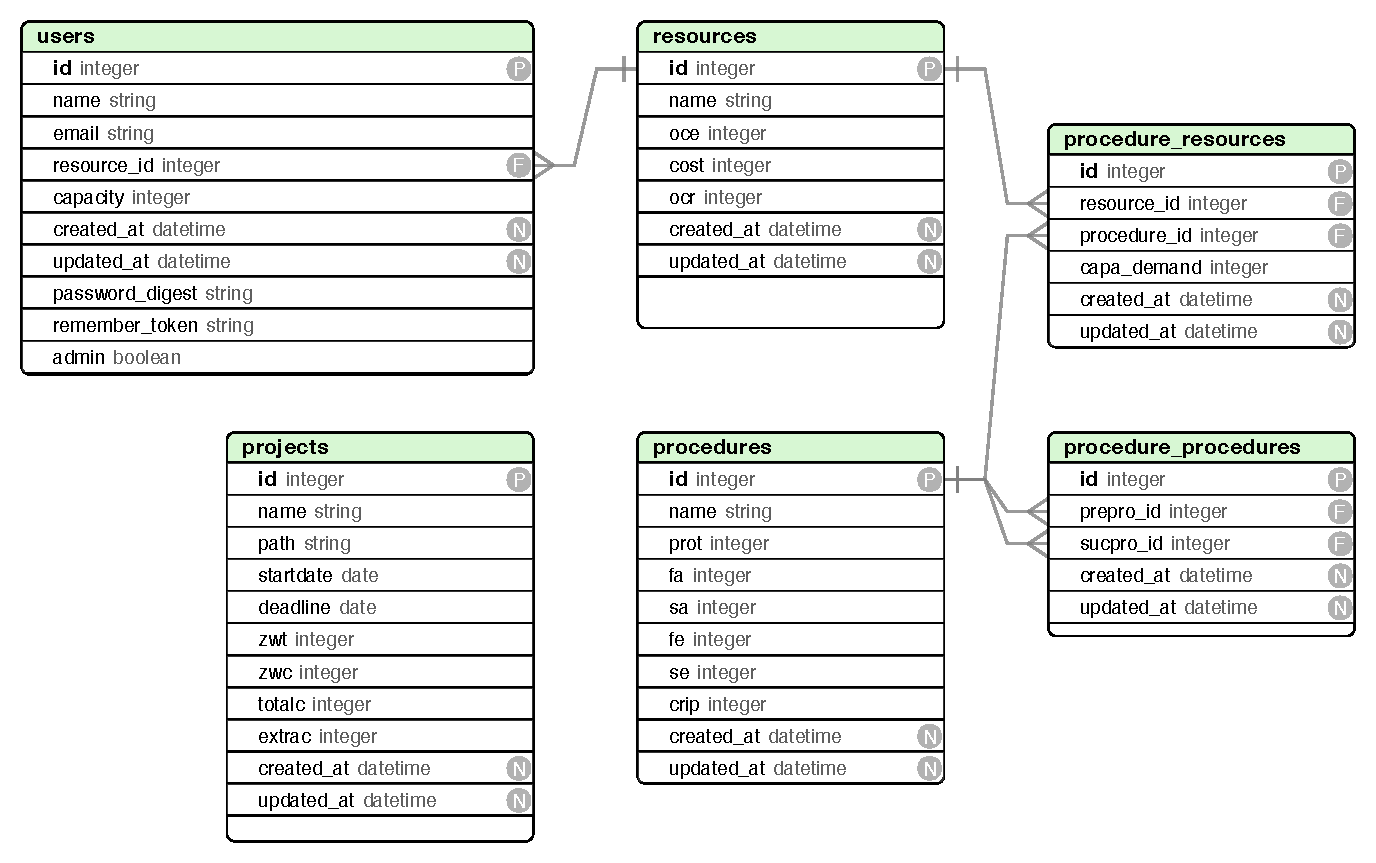
\includegraphics[width=150mm]{Bilder/DB.pdf}
    \caption{Datenbankschema der Web-Applikation Projektplanung}  \label{schema}
  \end{center}
\end{figure}

P = Primary Key, N = Not Null, D = Default Value

\subsection{GAMS-Implementierung des Beispiels}\label{Imp}
%\lstinputlisting[language=ruby, firstline=37, lastline=45, caption=Name, style=Listing]{/Users/Superuser/as-rcpsp/RCPSP1.gms}
\lstinputlisting[language=ruby, caption=GAMS-Code zur Kapazitätsplanung, style=Listing, label=rcpsp1]{/Users/Superuser/as-rcpsp/RCPSP1.gms}

\lstinputlisting[language=ruby, caption=GAMS-Code zur Kostenplanung, style=Listing, label=rcpsp2]{/Users/Superuser/as-rcpsp/RCPSP2.gms}


%%%%%%%%%RoR Codes%%%%%%%%%%%%%%%%%%%%%%%%%%%%%
\subsection{Ruby on Rails Programmcodes}\label{rcodes}

%%%%%%GEMFILIE
\lstinputlisting[language=ruby, caption=Gemfile der Web-Applikation Projektplanung, style=Listing, label=gemfile]{/Users/Superuser/as-rcpsp/Gemfile}

%%%%%%%routes
\lstinputlisting[language=ruby, caption=Routes-Datei der Web-Applikation Projektplanung, style=Listing, label=routes]{/Users/Superuser/as-rcpsp/config/routes.rb}

%%%%%%%%%%%%%Controller
\lstinputlisting[language=ruby, caption=RoR-Controller für die Vorgangsrelationen, style=Listing, label=ppc]{/Users/Superuser/as-rcpsp/app/controllers/procedure_procedures_controller.rb}

\lstinputlisting[language=ruby, caption=RoR-Controller für die Vorgangs-Ressourcen-Kombinationen, style=Listing]{/Users/Superuser/as-rcpsp/app/controllers/procedure_resources_controller.rb}

\lstinputlisting[language=ruby, caption=RoR-Controller für die Vorgänge, style=Listing]{/Users/Superuser/as-rcpsp/app/controllers/procedures_controller.rb}

\lstinputlisting[language=ruby, caption=RoR-Controller für das Projekt, style=Listing]{/Users/Superuser/as-rcpsp/app/controllers/projects_controller.rb}

\lstinputlisting[language=ruby, caption=RoR-Controller für das RCPSP, style=Listing, label=rcpspc]{/Users/Superuser/as-rcpsp/app/controllers/rcpsps_controller.rb}

\lstinputlisting[language=ruby, caption=RoR-Controller für die Ressourcen, style=Listing]{/Users/Superuser/as-rcpsp/app/controllers/resources_controller.rb}

\lstinputlisting[language=ruby, caption=RoR-Controller für die statischen Seiten, style=Listing, label=spc]{/Users/Superuser/as-rcpsp/app/controllers/static_pages_controller.rb}

\lstinputlisting[language=ruby, caption=RoR-Controller für die Users, style=Listing]{/Users/Superuser/as-rcpsp/app/controllers/users_controller.rb}

%%%%MODELS
\lstinputlisting[language=ruby, caption=RoR-Modell für die Vorgangsrelationen, style=Listing]{/Users/Superuser/as-rcpsp/app/models/procedure_procedure.rb}

\lstinputlisting[language=ruby, caption=RoR-Modell für die Vorgangs-Ressourcen-Kombinationen, style=Listing, label=prm]{/Users/Superuser/as-rcpsp/app/models/procedure_resource.rb}

\lstinputlisting[language=ruby, caption=RoR-Modell für die Vorgänge, style=Listing]{/Users/Superuser/as-rcpsp/app/models/procedure.rb}

\lstinputlisting[language=ruby, caption=RoR-Modell für das Projekt, style=Listing]{/Users/Superuser/as-rcpsp/app/models/project.rb}

\lstinputlisting[language=ruby, caption=RoR-Modell für die Ressourcen, style=Listing]{/Users/Superuser/as-rcpsp/app/models/resource.rb}

\lstinputlisting[language=ruby, caption=RoR-Modell für die Users, style=Listing, label=fehler_code]{/Users/Superuser/as-rcpsp/app/models/user.rb}

%%%VIEWS propro
\lstinputlisting[language=ruby, caption=RoR-Seite für die Vorgangsrelationen - Formular, style=Listing]{/Users/Superuser/as-rcpsp/app/views/procedure_procedures/_form.html.erb}

\lstinputlisting[language=ruby, caption=RoR-Seite für die Vorgangsrelationen - Übersicht, style=Listing]{/Users/Superuser/as-rcpsp/app/views/procedure_procedures/index.html.erb}

\lstinputlisting[language=ruby, caption=RoR-Seite für die Vorgangsrelationen - Erstellung, style=Listing]{/Users/Superuser/as-rcpsp/app/views/procedure_procedures/new.html.erb}

\lstinputlisting[language=ruby, caption=RoR-Seite für die Vorgangsrelationen - Grafische Darstellung, style=Listing, label=graphv]{/Users/Superuser/as-rcpsp/app/views/procedure_procedures/graph.html.erb}

%%%VIEWS prores
\lstinputlisting[language=ruby, caption=RoR-Seite für die Vorgangs-Ressourcen-Kombinationen - Formular, style=Listing]{/Users/Superuser/as-rcpsp/app/views/procedure_resources/_form.html.erb}

\lstinputlisting[language=ruby, caption=RoR-Seite für die Vorgangs-Ressourcen-Kombinationen - Bearbeitung, style=Listing]{/Users/Superuser/as-rcpsp/app/views/procedure_resources/edit.html.erb}

\lstinputlisting[language=ruby, caption=RoR-Seite für die Vorgangs-Ressourcen-Kombinationen - Übersicht, style=Listing]{/Users/Superuser/as-rcpsp/app/views/procedure_resources/index.html.erb}

\lstinputlisting[language=ruby, caption=RoR-Seite für die Vorgangs-Ressourcen-Kombinationen - Erstellung, style=Listing]{/Users/Superuser/as-rcpsp/app/views/procedure_resources/new.html.erb}

\lstinputlisting[language=ruby, caption=RoR-Seite für die Vorgangs-Ressourcen-Kombinationen - Anzeige, style=Listing]{/Users/Superuser/as-rcpsp/app/views/procedure_resources/show.html.erb}

%%%VIEWS pro
\lstinputlisting[language=ruby, caption=RoR-Seite für die Vorgänge - Formular, style=Listing]{/Users/Superuser/as-rcpsp/app/views/procedures/_form.html.erb}

\lstinputlisting[language=ruby, caption=RoR-Seite für die Vorgänge - Bearbeitung, style=Listing]{/Users/Superuser/as-rcpsp/app/views/procedures/edit.html.erb}

\lstinputlisting[language=ruby, caption=RoR-Seite für die Vorgänge - Übersicht, style=Listing]{/Users/Superuser/as-rcpsp/app/views/procedures/index.html.erb}

\lstinputlisting[language=ruby, caption=RoR-Seite für die Vorgänge - Erstellung, style=Listing]{/Users/Superuser/as-rcpsp/app/views/procedures/new.html.erb}

\lstinputlisting[language=ruby, caption=RoR-Seite für die Vorgänge - Anzeige, style=Listing]{/Users/Superuser/as-rcpsp/app/views/procedures/show.html.erb}

%%%VIEWS res
\lstinputlisting[language=ruby, caption=RoR-Seite für die Ressourcen - Formular, style=Listing]{/Users/Superuser/as-rcpsp/app/views/resources/_form.html.erb}

\lstinputlisting[language=ruby, caption=RoR-Seite für die Ressourcen - Tabelle als unangemeldeter User, style=Listing]{/Users/Superuser/as-rcpsp/app/views/resources/_free.html.erb}

\lstinputlisting[language=ruby, caption=RoR-Seite für die Ressourcen - Tabelle als angemeldeter User, style=Listing, label=sign_res]{/Users/Superuser/as-rcpsp/app/views/resources/_signed_in.html.erb}

\lstinputlisting[language=ruby, caption=RoR-Seite für die Ressourcen - Bearbeitung, style=Listing]{/Users/Superuser/as-rcpsp/app/views/resources/edit.html.erb}

\lstinputlisting[language=ruby, caption=RoR-Seite für die Ressourcen - Übersicht, style=Listing, label=index_res]{/Users/Superuser/as-rcpsp/app/views/resources/index.html.erb}

\lstinputlisting[language=ruby, caption=RoR-Seite für die Ressourcen - Erstellung, style=Listing]{/Users/Superuser/as-rcpsp/app/views/resources/new.html.erb}

\lstinputlisting[language=ruby, caption=RoR-Seite für die Ressourcen - Anzeige, style=Listing]{/Users/Superuser/as-rcpsp/app/views/resources/show.html.erb}

%%%VIEWS static
\lstinputlisting[language=ruby, caption=RoR-Seite für die Optimierungsseite zur Projektplanung, style=Listing]{/Users/Superuser/as-rcpsp/app/views/static_pages/rcpsp.html.erb}

\lstinputlisting[language=ruby, caption=RoR-Seite für die Startseite, style=Listing, label=test]{/Users/Superuser/as-rcpsp/app/views/static_pages/home.html.erb}

\lstinputlisting[language=ruby, caption=Kopfzeile der Web-Apllikation, style=Listing, label=header]{/Users/Superuser/as-rcpsp/app/views/layouts/_header.html.erb}


%%%VIEWS user
\lstinputlisting[language=ruby, caption=RoR-Seite bzgl. der Lösung von Usern über die Übersichtsseite, style=Listing]{/Users/Superuser/as-rcpsp/app/views/users/_user.html.erb}

\lstinputlisting[language=ruby, caption=RoR-Seite für die User - Bearbeitung, style=Listing]{/Users/Superuser/as-rcpsp/app/views/users/edit.html.erb}

\lstinputlisting[language=ruby, caption=RoR-Seite für die User - User-/Mitarbeiterübersicht, style=Listing]{/Users/Superuser/as-rcpsp/app/views/users/index.html.erb}

\lstinputlisting[language=ruby, caption=RoR-Seite für die User - Erstellung, style=Listing]{/Users/Superuser/as-rcpsp/app/views/users/new.html.erb}

\lstinputlisting[language=ruby, caption=RoR-Seite für die User - Anzeige, style=Listing, label=show_user]{/Users/Superuser/as-rcpsp/app/views/users/show.html.erb}

%%%schema
\lstinputlisting[language=ruby, caption=RoR-Datenbankschema, style=Listing]{/Users/Superuser/as-rcpsp/db/schema.rb}

%%%sample
\lstinputlisting[language=ruby, caption=Beispieldaten für die Datenbank, style=Listing]{/Users/Superuser/as-rcpsp/lib/tasks/sample_data.rake}

%%%datepicker
%\lstinputlisting[language=java, caption=JavaScrip-Datei zum Datepicker, style=Listing2]{/Users/Superuser/as-rcpsp/vendor/assets/javascripts/bootstrap-datepicker/core.js}

\end{appendix}
\end{document}
%%%%%%%%%%%%%%%%%%%%%%%%%%ENDE%%%%%%%%%%%%%%%%%%%

